%&pdflatex
\chapter{Installazione}\label{ch:install}
In questo capitolo seguiremo passo passo la procedura di installazione di Debian, accompagnando la trattazione con qualche \textit{screenshot}.

Durante tutta l'installazione, per una buona riuscita, è fondamentale leggere e comprendere tutto ciò che l'installer di Debian mostra sullo schermo. Quindi, ad ogni passaggio, si raccomanda di fermarsi e leggere quanto compare sullo schermo prima di intraprendere qualsiasi azione.
%&pdflatex
\section{Impostazione della lingua}
La prima schermata che ci darà l'installer di Debian è mostrata in Figura \vref{fig:language-selection}.

\begin{figure}[ht]
	\centering
	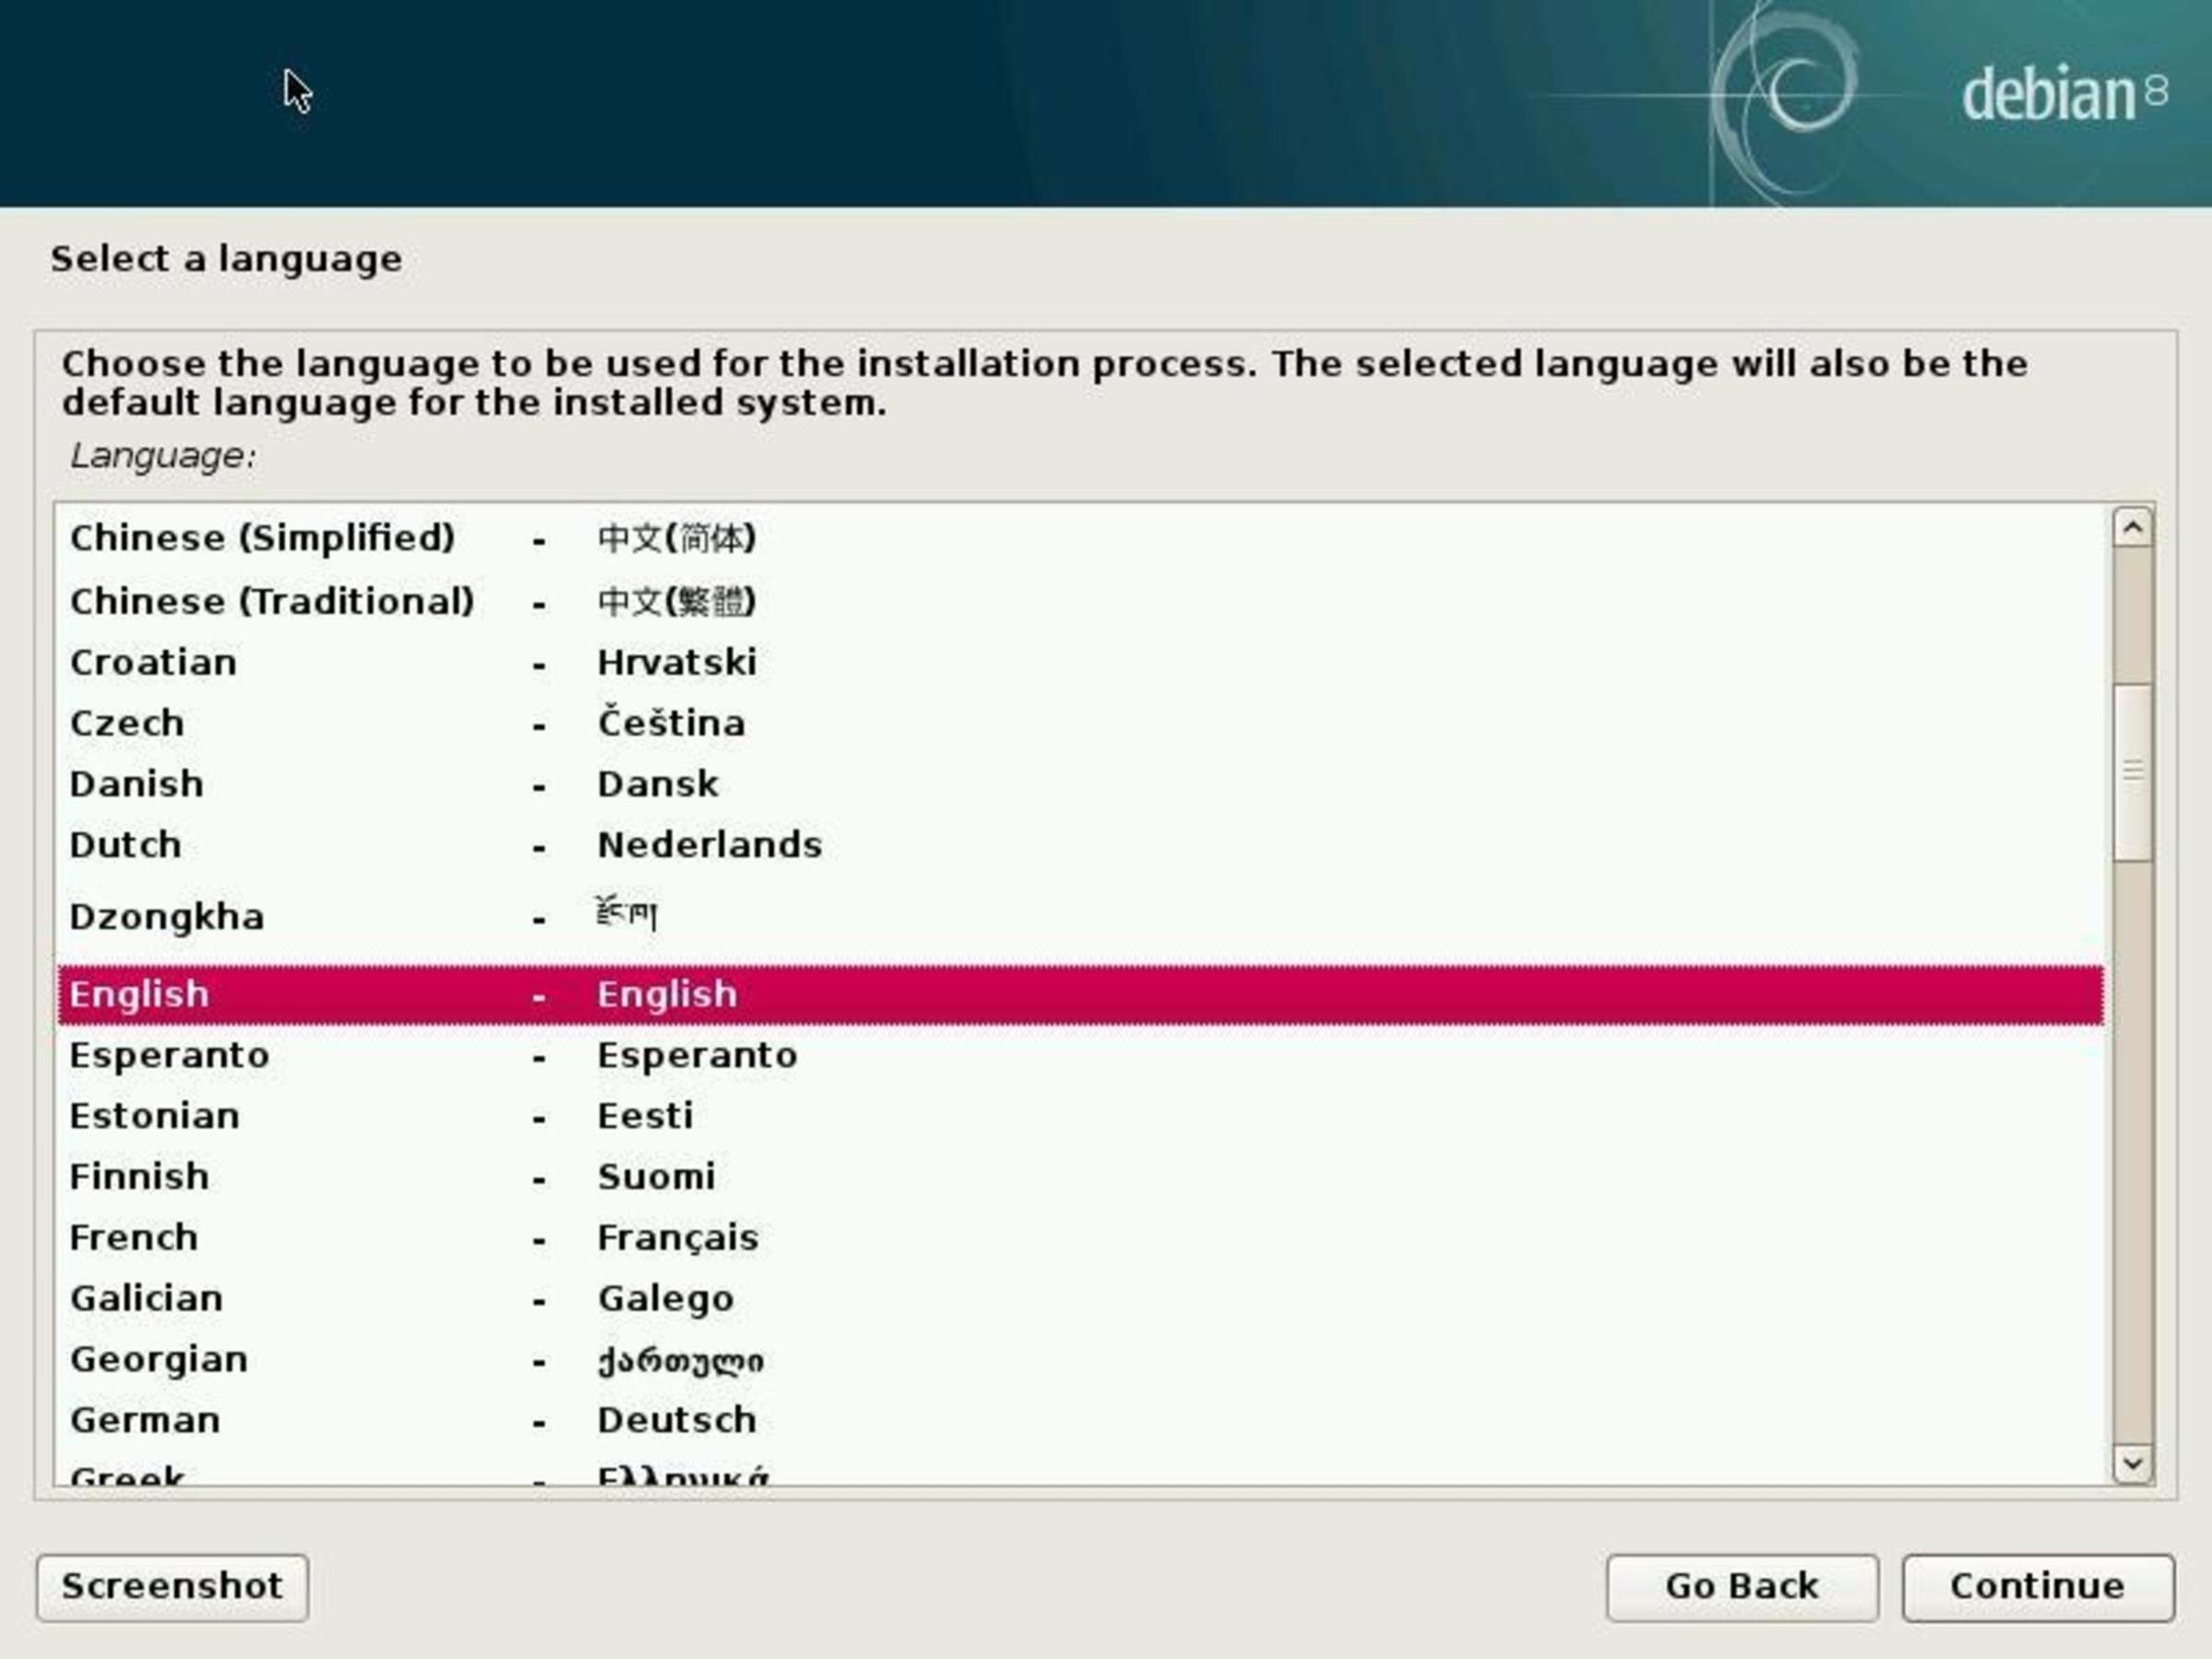
\includegraphics[resolution=600]{language-selection}
	\caption{Selezione della lingua}
	\label{fig:language-selection}
\end{figure}

Tra le lingue è disponibile anche l'italiano. Consigliamo però, se non si hanno problemi con la lingua inglese, di selezionare l'inglese: in tal modo in caso di problemi con il software, i \textit{log} dei programmi saranno mostrati in lingua inglese, permettendo quindi di chiedere assistenza nelle community internazionali di Linux mostrando i log in inglese. Ad ogni modo, il lettore può scegliere \texttt{Italiano} se preferisce. Una volta scelta la lingua, cliccare su \texttt{Continue}.

Nella schermata successiva viene chiesto di scegliere la propria zona per impostare correttamente l'ora secondo il fuso orario locale. Se al passaggio precedente si è scelto la lingua italiana, dovrebbe essere adesso comparsa la voce \texttt{Italia}. Se invece si è scelto, come consigliato, la lingua inglese, allora è necessario selezionare in ordine: \texttt{other} (in fondo alla lista) > \texttt{Europe} > \texttt{Italy}.

Successivamente, se si è scelto come lingua l'inglese e come zona l'Italia, l'installer ci chiederà quale locale utilizzare. Scegliamo \texttt{United States - en\_US.UTF-8} come mostrato in Figura \vref{fig:locale-selection}.

\begin{figure}[ht]
	\centering
	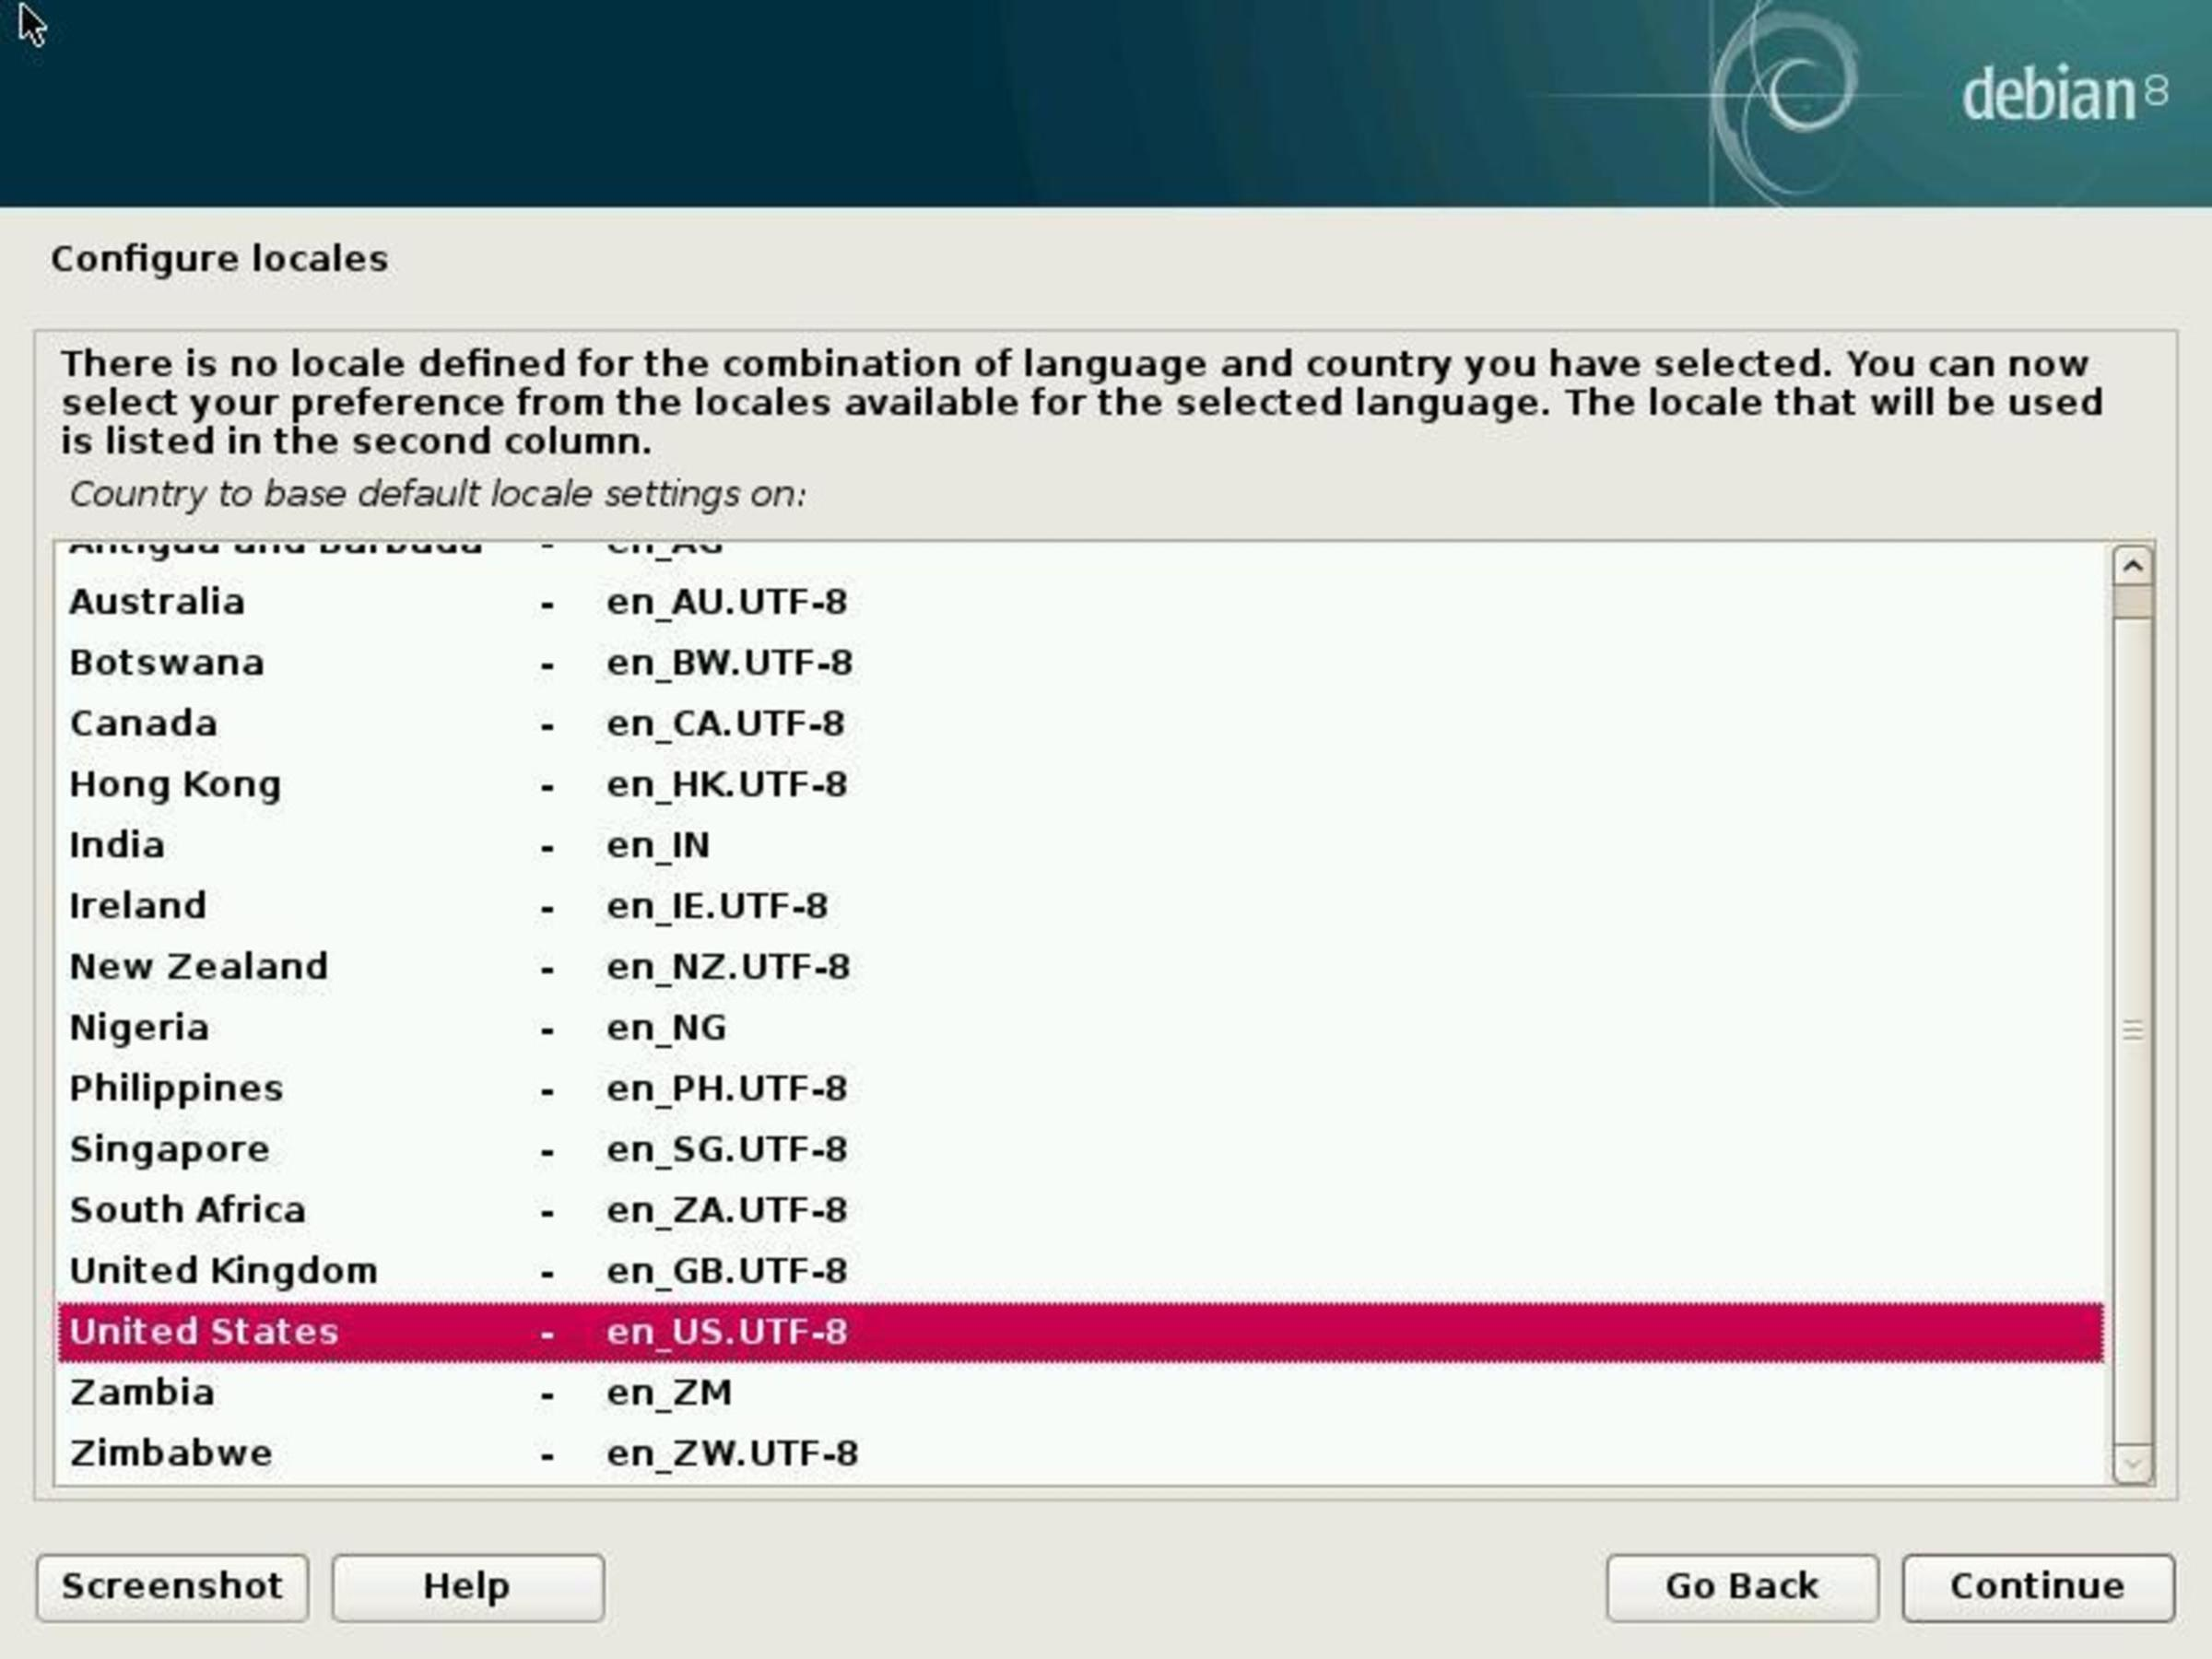
\includegraphics[resolution=600]{locale-selection}
	\caption{Selezione del locale}
	\label{fig:locale-selection}
\end{figure}

Se invece si è scelto come lingua l'italiano e come zona l'Italia, verrà selezionato automaticamente \texttt{Italia - it\_IT.UTF-8}.

Infine, ci verrà chiesto di selezionare il \textit{layout di tastiera}. Scegliamo \texttt{Italian} (\texttt{Italiana}).

%&pdflatex
\section{Configurazione di rete}
Se il lettore ha seguito il consiglio che avevamo dato nel paragrafo \vref{sec:starting-debian} di attaccare il cavo Ethernet al proprio computer, Debian dovrebbe aver effettuato la configurazione automatica della rete. Se ciò non è successo, è necessario configurarla manualmente seguendo la procedura guidata che non verrà trattata in questo testo.

A questo punto Debian ci chiederà di impostare l'\textit{hostname} della macchina (Figura \vref{fig:hostname-selection}).

\begin{figure}[ht]
	\centering
	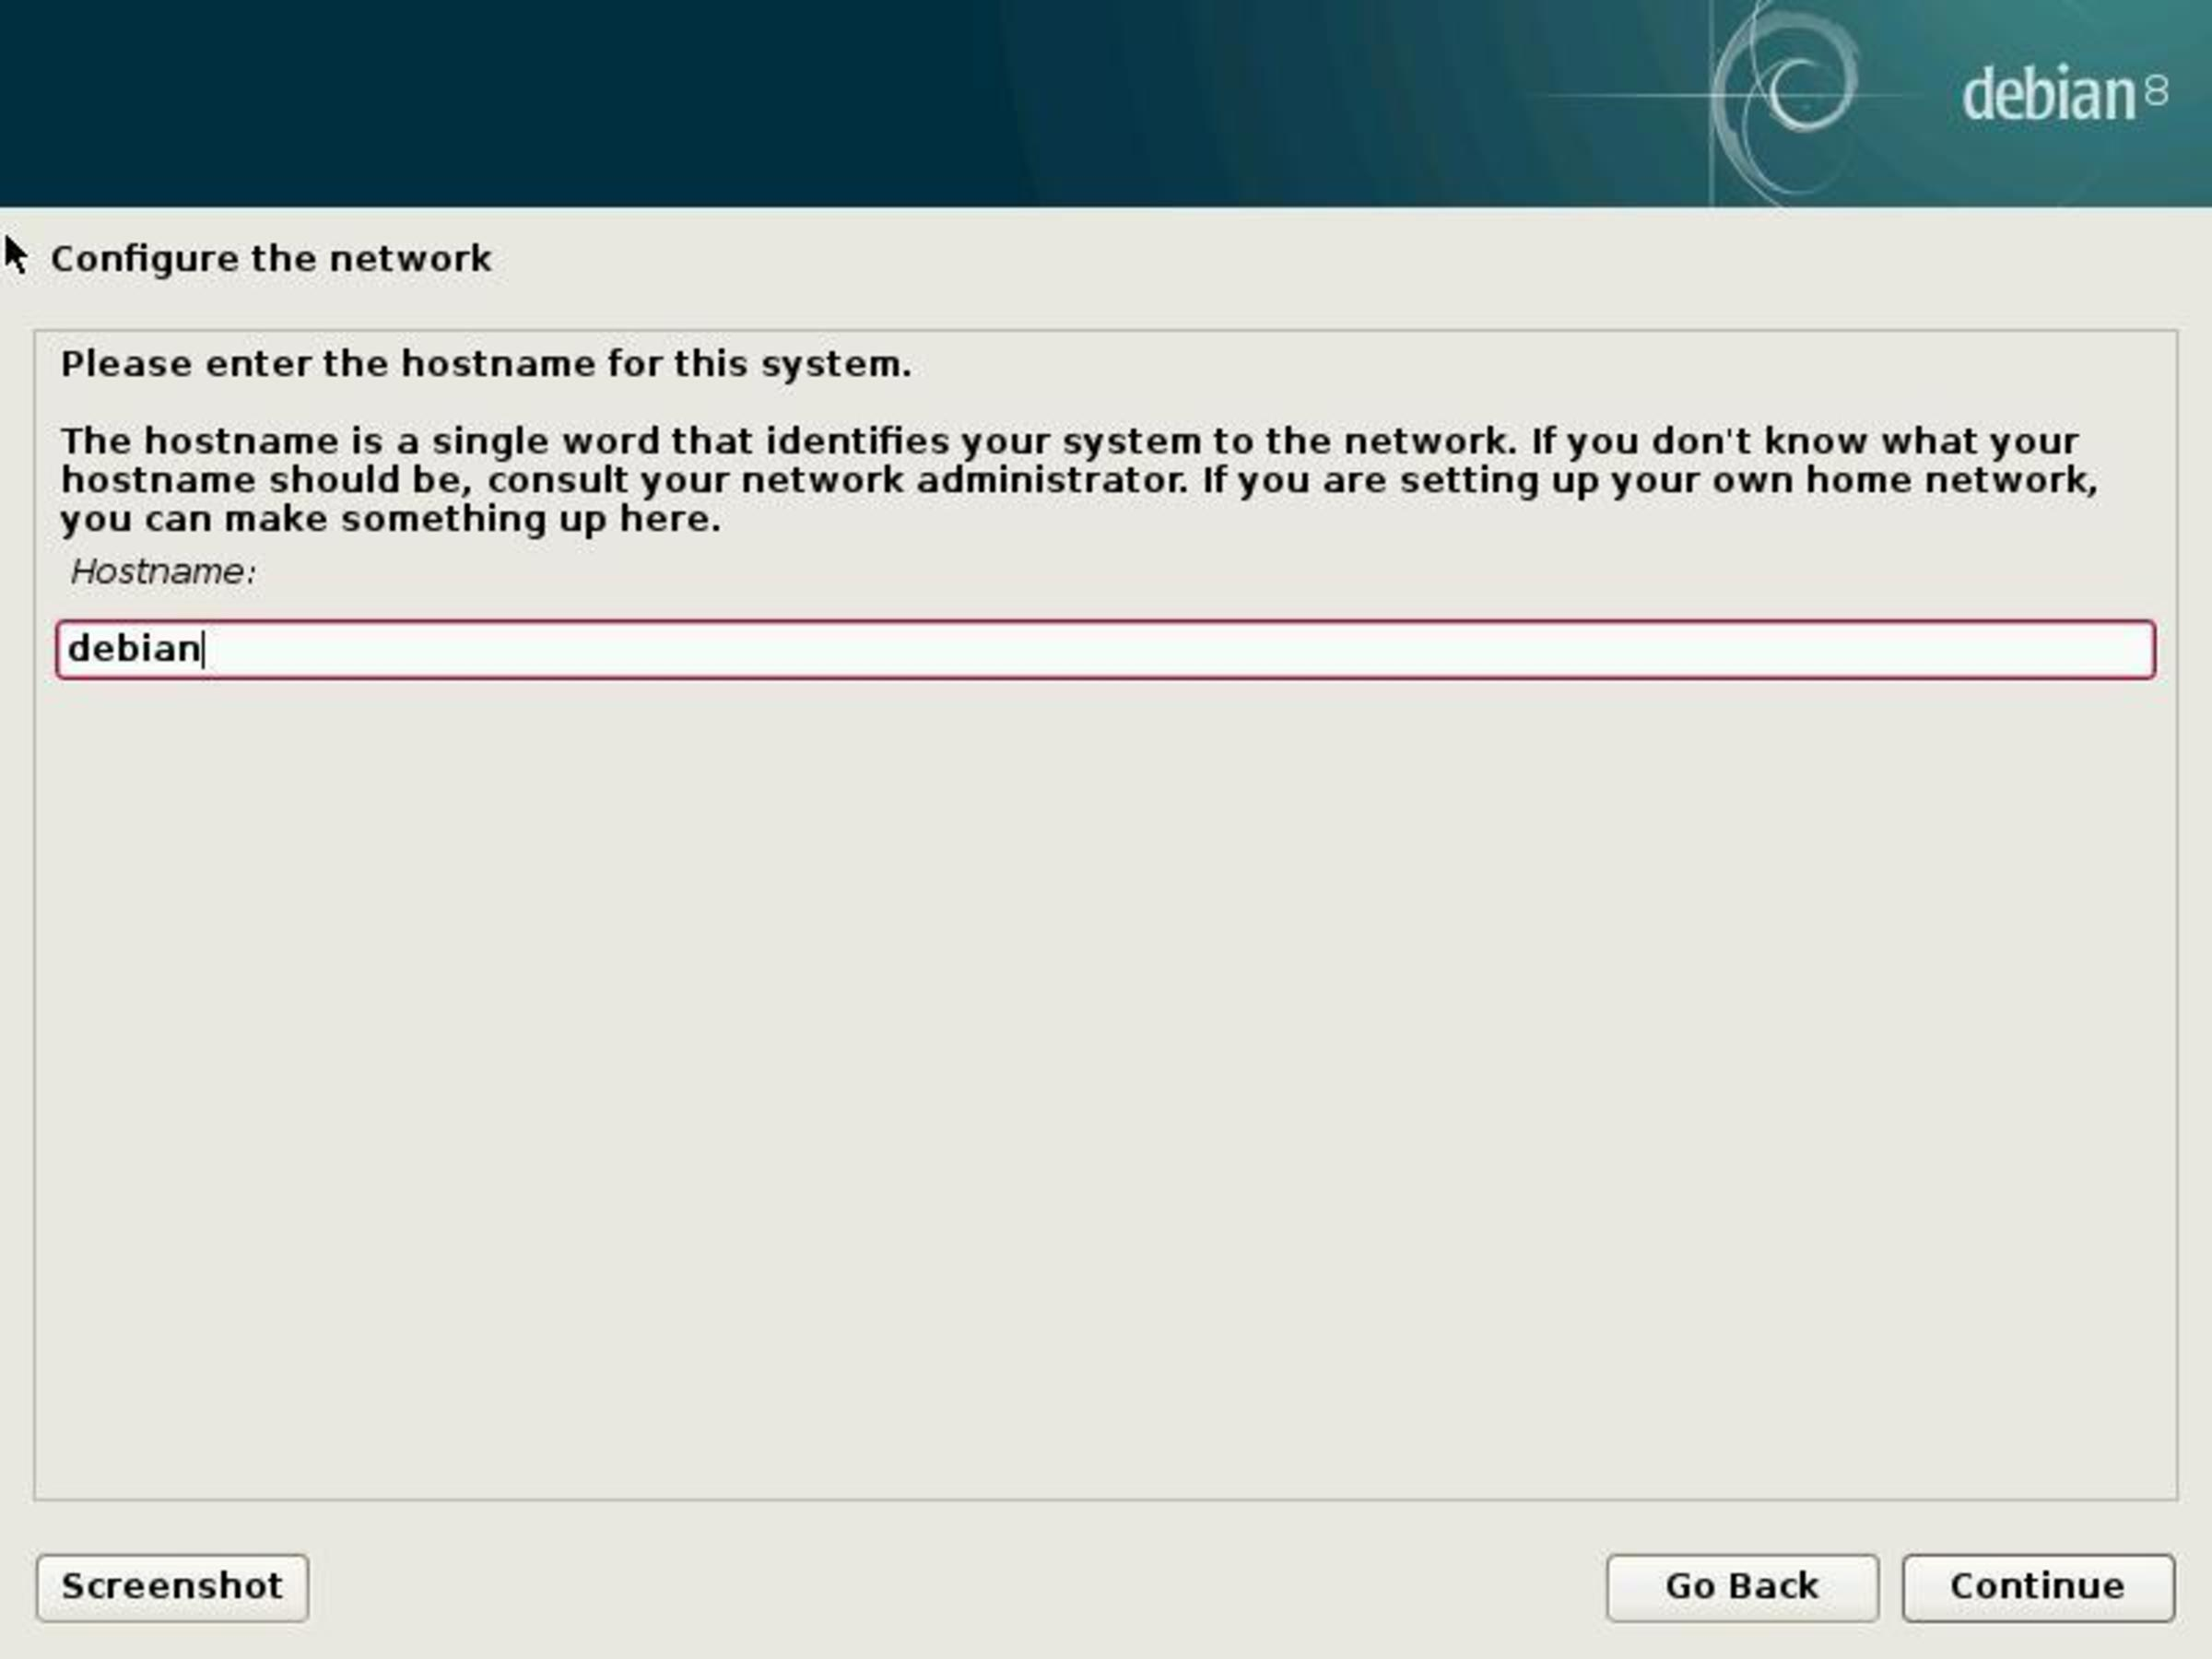
\includegraphics[resolution=600]{hostname-selection}
	\caption{Selezione di un hostname}
	\label{fig:hostname-selection}
\end{figure}

L'hostname è ciò che in Windows viene chiamato \textit{"nome del PC"}. È possibile scegliere qualsiasi cosa come hostname: solitamente, per evitare problemi con alcune applicazioni, si imposta \texttt{localhost} --- ma anche \texttt{debian} va bene, o qualsiasi altra cosa.

Dopodiché, Debian ci chiederà di impostare il dominio da appendere all'hostname. Solitamente questo campo si lascia vuoto, ma anche qui si può scegliere qualsiasi cosa.

%&pdflatex
\section{Impostazione degli utenti}
Linux è un sistema \textit{multi-utente}. Esiste, in ogni sistema Linux, un \textit{utente amministratore} con privilegi massimi sul sistema chiamato \texttt{root}. Il prossimo passo è impostare la password dell'account amministratore \texttt{root} (Figura \vref{fig:root-password}).

\begin{figure}[ht]
	\centering
	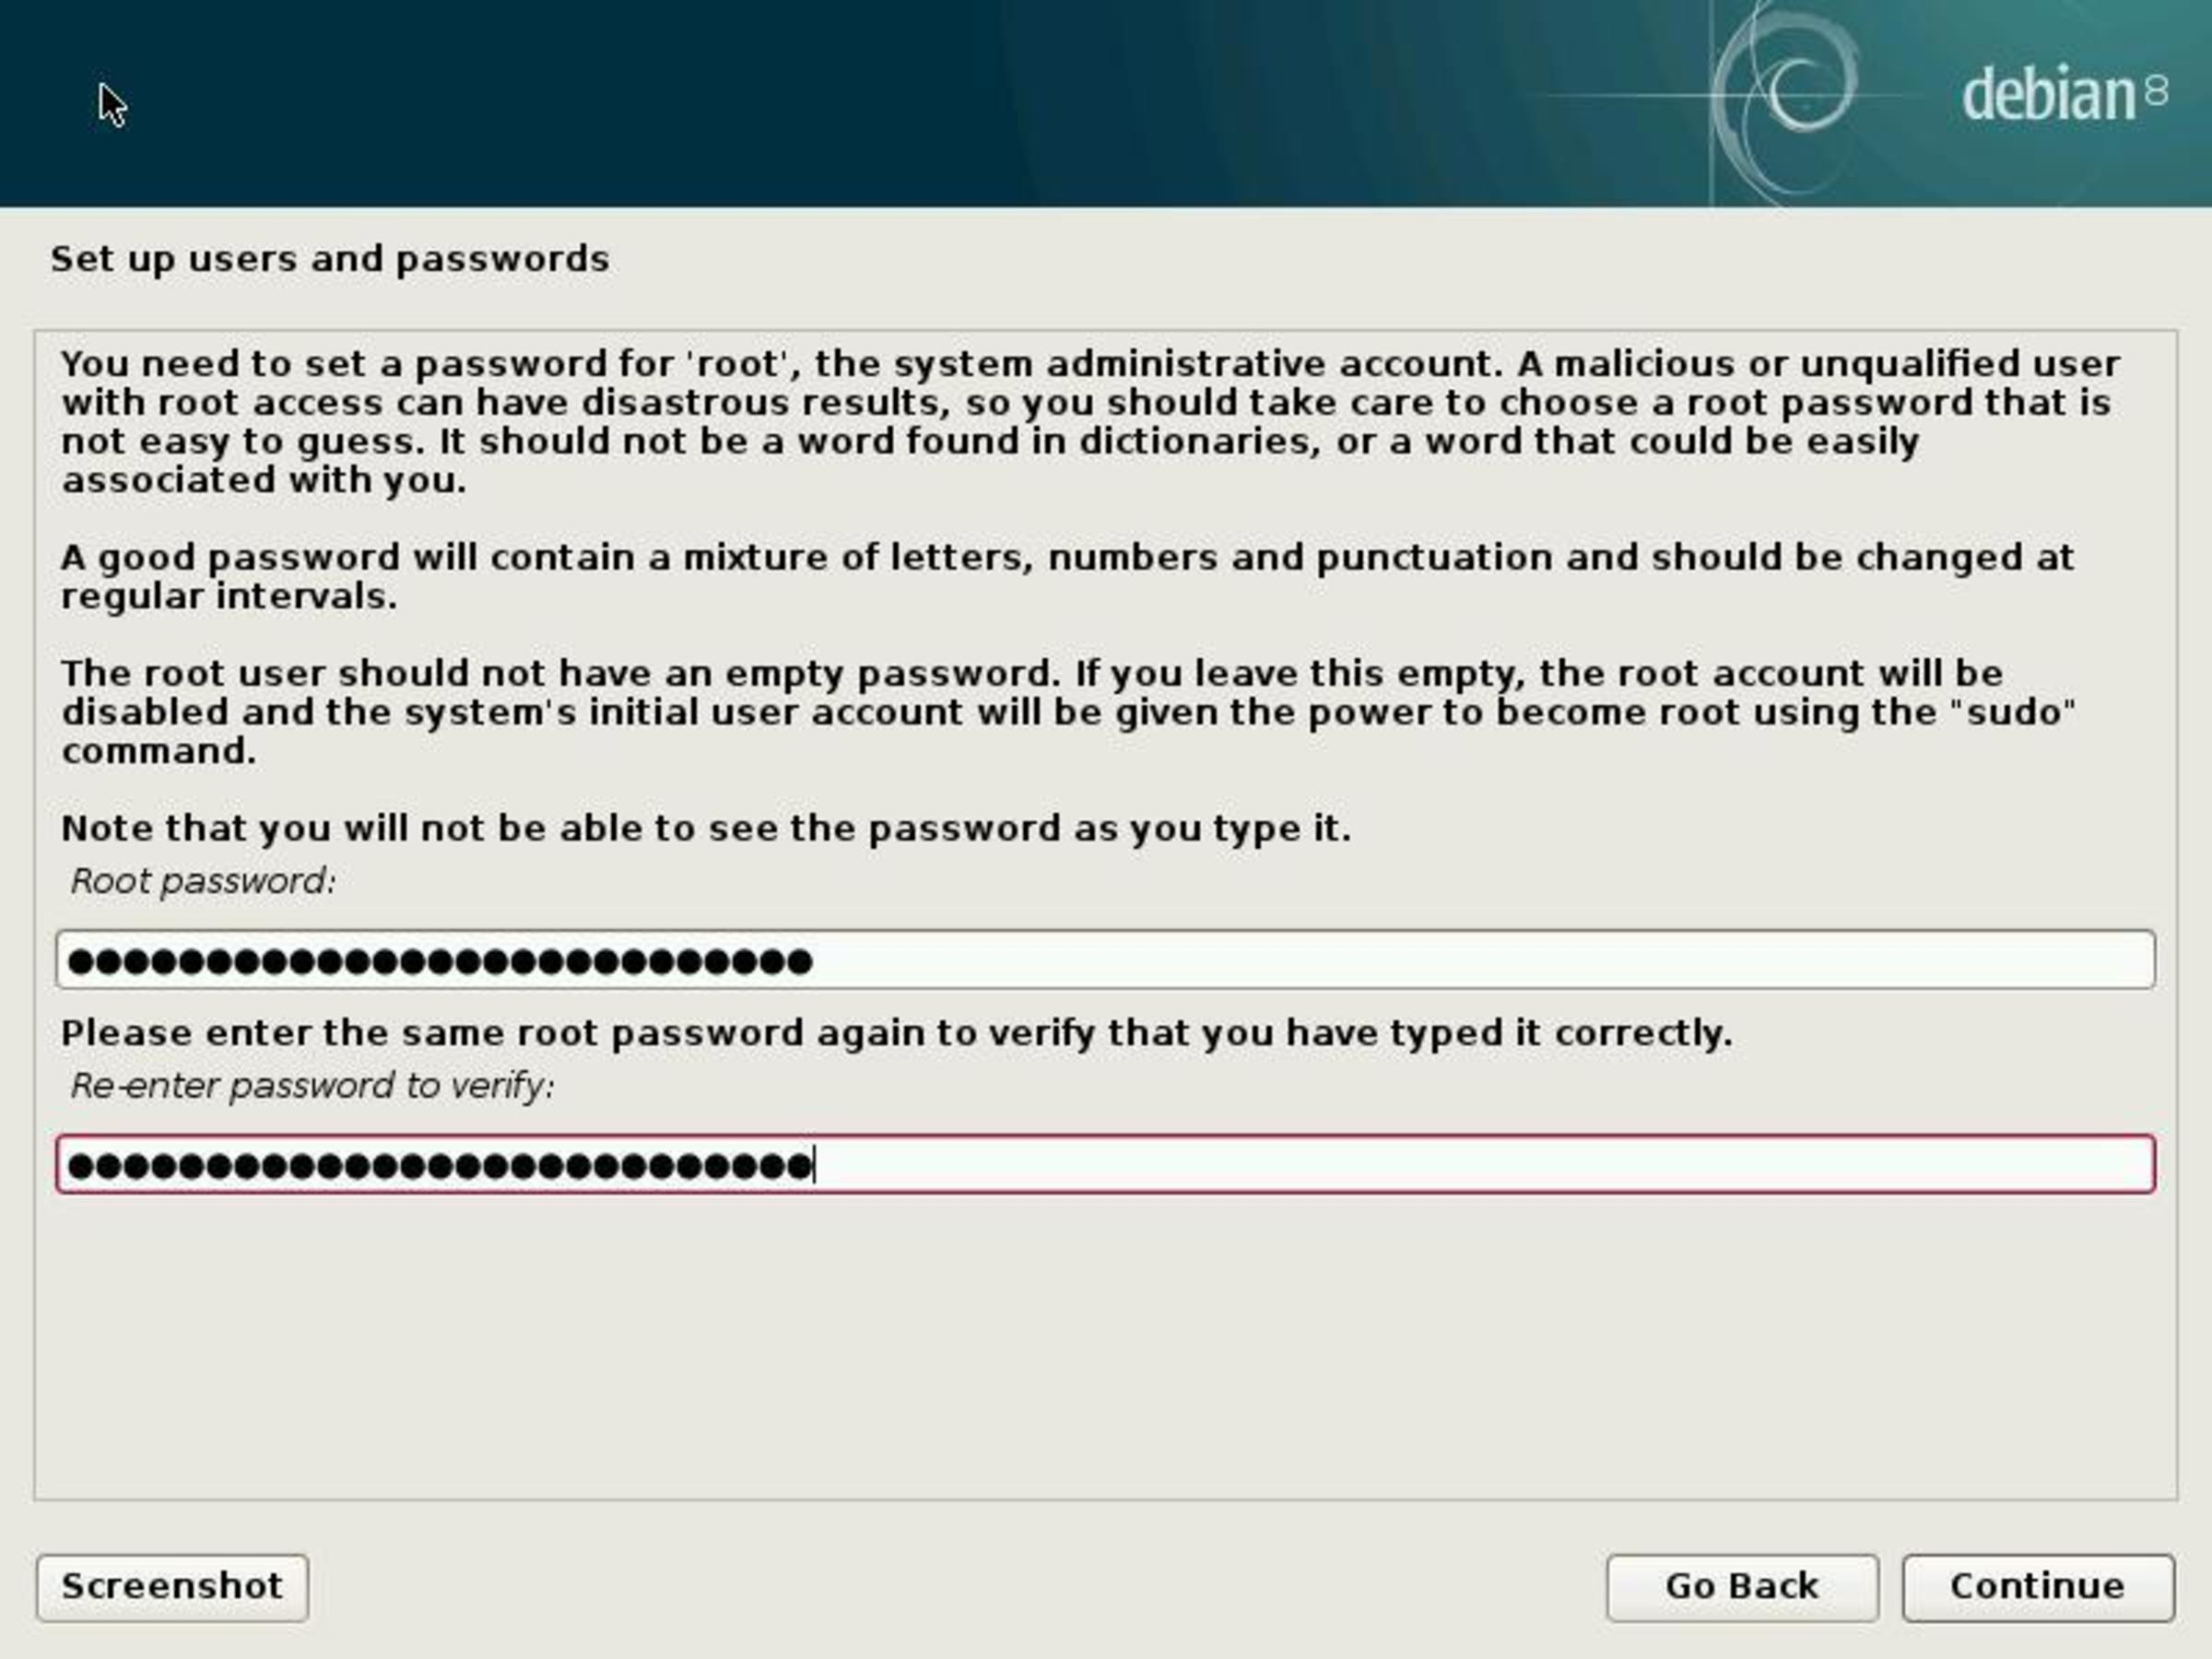
\includegraphics[resolution=600]{root-password}
	\caption{Impostazione della password dell'account \texttt{root}}
	\label{fig:root-password}
\end{figure}

La password non dovrebbe essere troppo semplice da indovinare e dovrebbe essere sufficientemente lunga e sicura. Bisogna tenere presente che una persona che ha accesso come \texttt{root} a un sistema Linux può anche, ad esempio, cancellare tutti i file (sistema operativo compreso) presenti nel disco!

Successivamente, ci verrà chiesto di creare un nuovo \textit{utente standard}. Essendo pericoloso usare \texttt{root} per le attività quotidiane (se si scarica uno \textit{script} contenente \texttt{rm -rf -{}-no-preserve-root /} e si esegue utilizzando l'account \texttt{root} l'intero disco viene cancellato), viene solitamente creato un account personale con privilegi limitati: nel momento in cui sono necessari privilegi amministrativi, sarà sempre possibile accedere temporaneamente come \texttt{root}. Il primo passo è scegliere un \textit{nome completo}. Questo, dovrebbe essere il nome reale dell'utente (ad esempio \texttt{Niccolò Scatena}). Successivamente, sarà chiesto di inserire un \textit{username} che verrà usato per il login: l'username deve essere tutto minuscolo (ad esempio \texttt{speedjack}). Infine, bisogna scegliere la password del nuovo account (in genere, diversa da quella di \texttt{root}).

%&pdflatex
\section{Partizionamento del disco}
Questa è la parte più difficile (e pericolosa). Dobbiamo partizionare il disco per far spazio a Debian. Prima di tutto, bisogna scegliere che partizioni creare per Debian: possiamo farne una sola, che conterrà tutto il sistema operativo, i programmi, e i nostri dati; oppure più partizioni dove, ad esempio, una partizione contiene il sistema operativo e i programmi (partizione \texttt{root}, simbolo \texttt{/}) e un'altra i nostri dati personali (partizione \texttt{/home}); possiamo anche dividere ulteriormente il sistema in altre partizioni ancora (\texttt{/var}, \texttt{/tmp}, \texttt{/usr}, ecc.), ma non lo consigliamo. Nell'esempio di questo testo, divideremo Debian su due partizioni: la \texttt{root} (\texttt{/}) e la \texttt{/home}. Se però si preferisce, è possibile inserire anche tutto in un'unica partizione.

Dobbiamo anche decidere se utilizzare \texttt{LVM}, che permette in qualsiasi momento di ridimensionare le partizioni facilmente (si cerchi sul web per maggiori informazioni); e se cifrare il disco per evitare che qualcuno possa vedere i nostri dati semplicemente avviando una live sul sistema (si cerchi sul web per \textit{"LUKS"} per maggiori informazioni). Anche se è fortemente consigliato cifrare il disco per la sicurezza, la procedura (comunque semplice) non sarà vista in questo testo. Di seguito, ci limiteremo a partizionare il disco senza usare \texttt{LVM} e senza cifrare il disco.

\begin{figure}[ht]
	\centering
	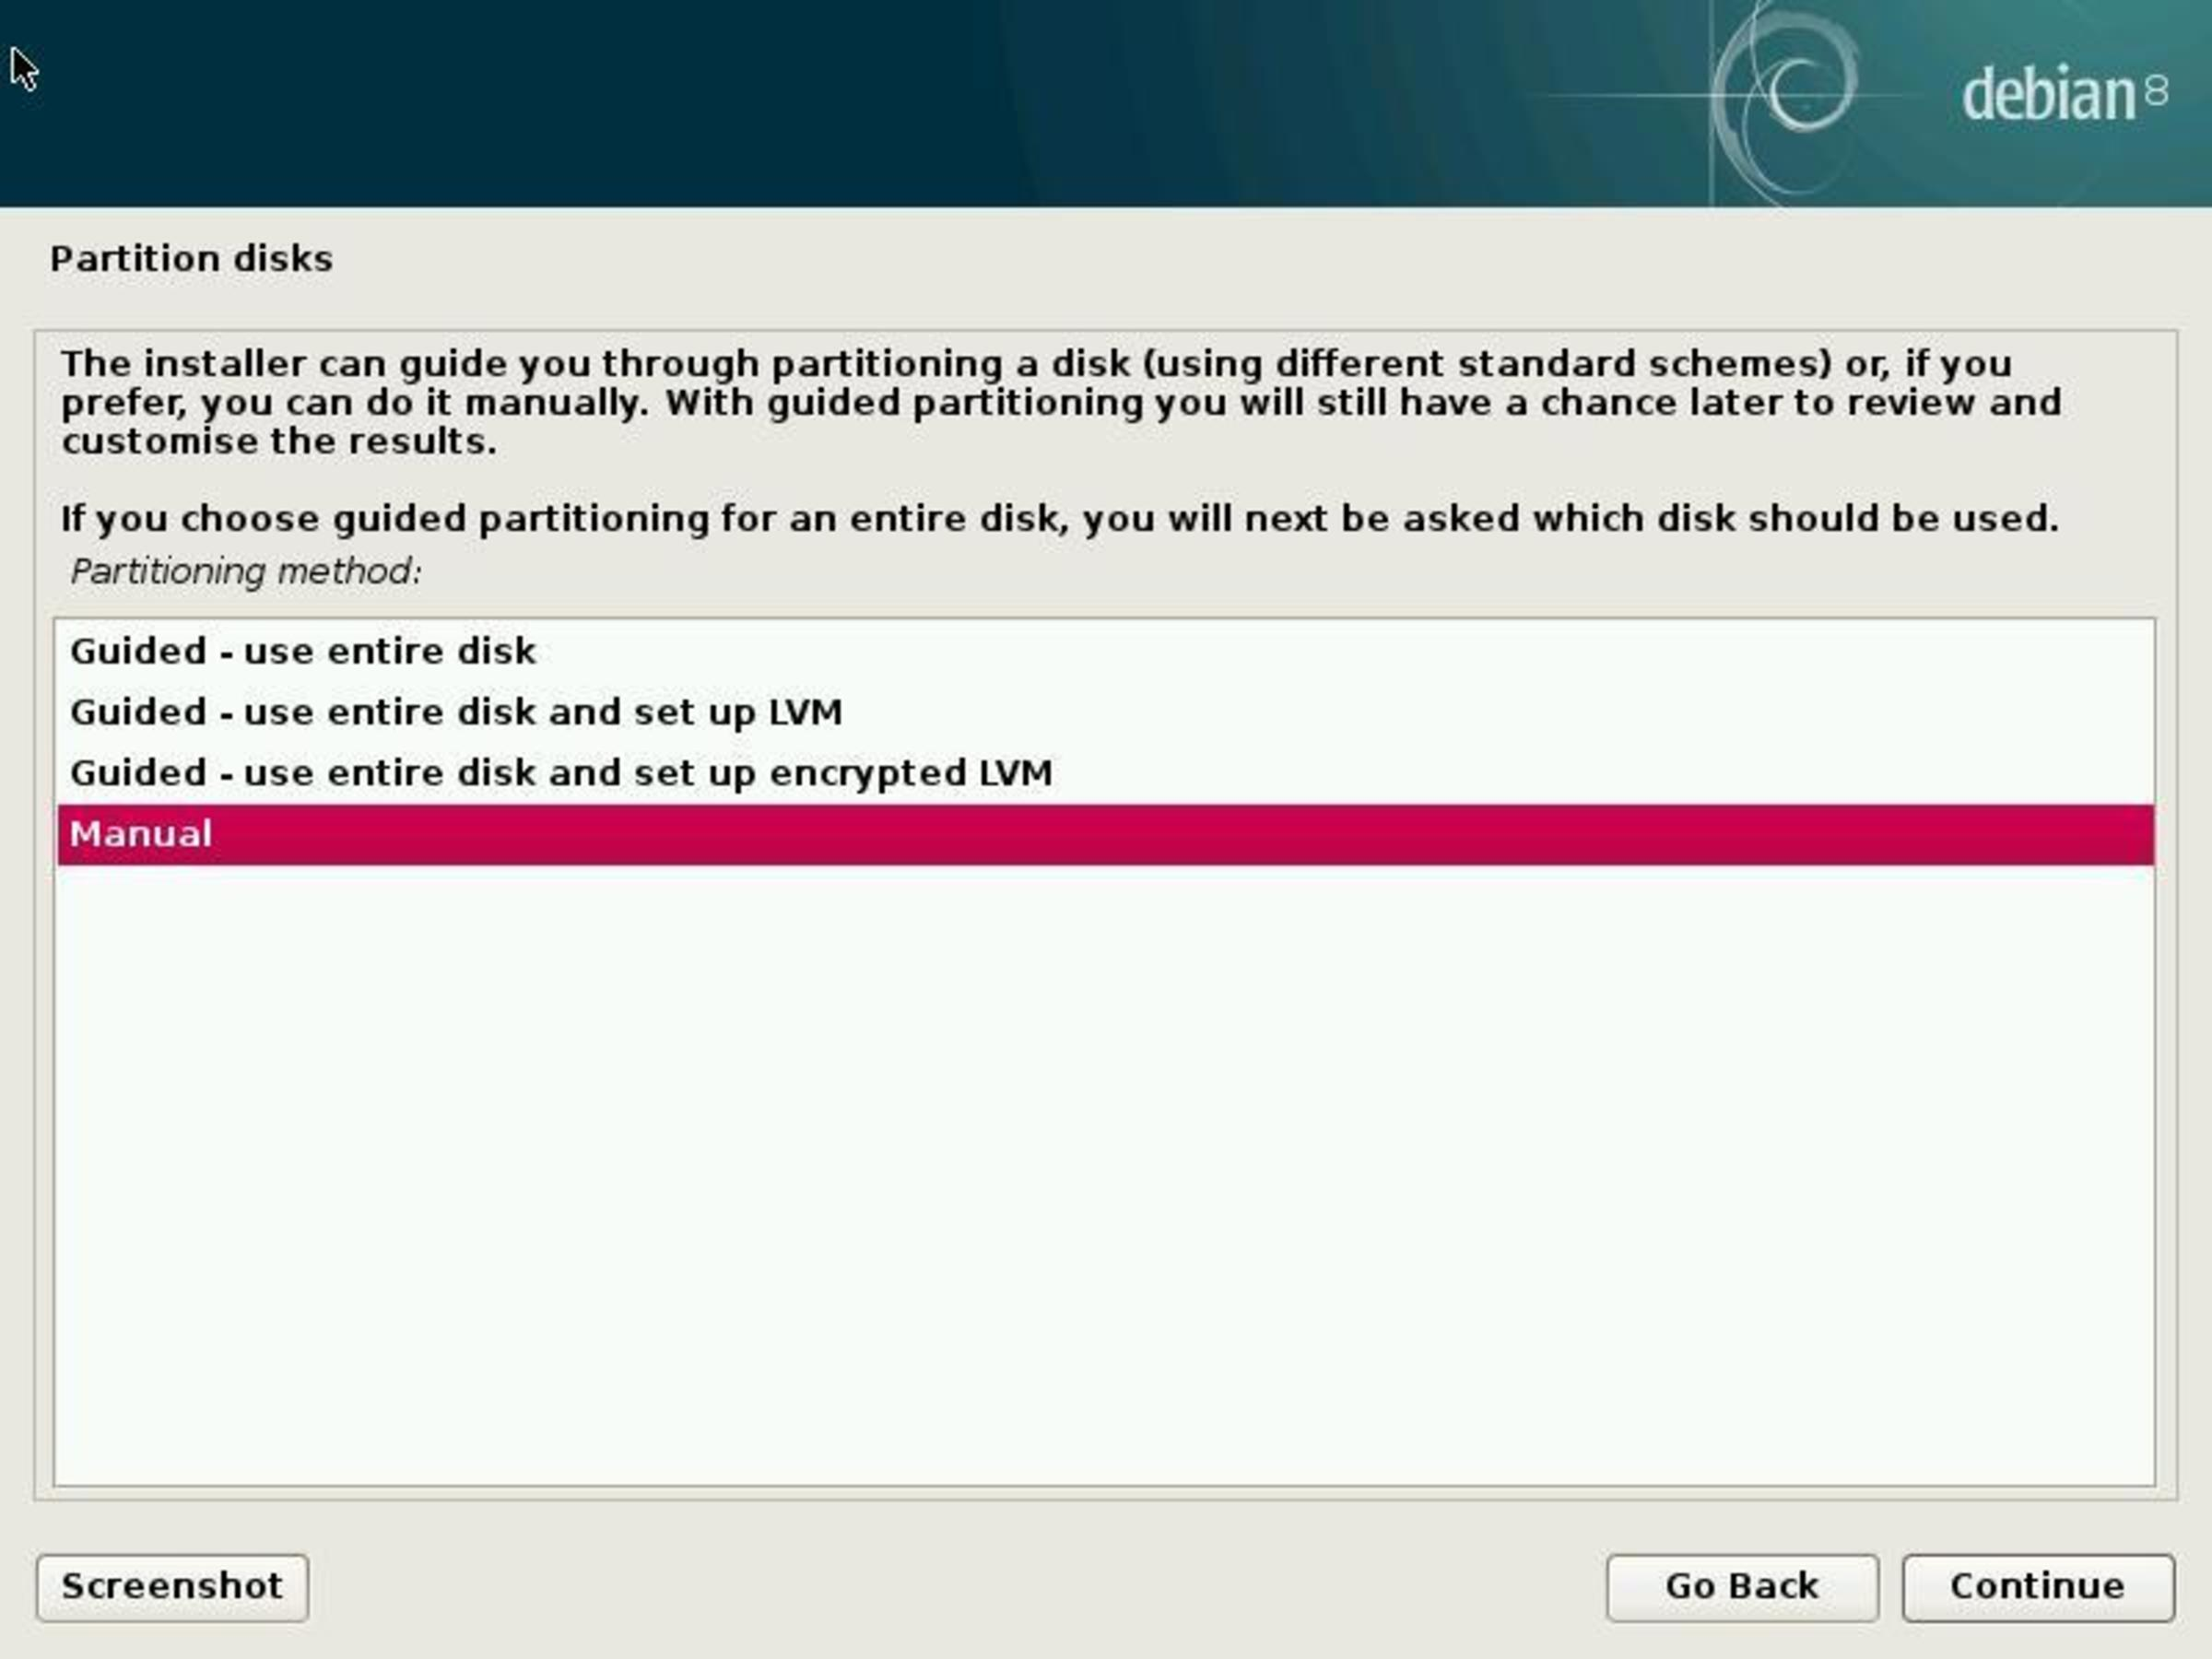
\includegraphics{manual-partitioning}
	\caption{Scelta del metodo di partizionamento: guidato o manuale}
	\label{fig:manual-partitioning}
\end{figure}

Inoltre, a questo punto, dobbiamo decidere se impostare un dual-boot con il sistema operativo già presente sul sistema (nell'esempio, Windows 10), oppure se sostituire il vecchio sistema operativo. Se vogliamo sostituire il vecchio sistema operativo, nella schermata di Figura \vref{fig:manual-partitioning} sceglieremo uno dei tre metodi guidati (\texttt{Guided}), in base al fatto se vogliamo anche impostare \texttt{LVM} e cifrare il disco. Dobbiamo scegliere la procedura guidata anche nel caso di installazione sotto macchina virtuale. Se scegliamo la procedura guidata, successivamente ci ritroveremo direttamente alla schermata di Figura \vref{fig:partitioning}.
Se invece vogliamo mantenere anche il vecchio sistema operativo e configurare un dual-boot, dobbiamo scegliere il metodo di partizionamento \texttt{Manuale} (\texttt{Manual}, in Figura \vref{fig:manual-partitioning}), e ridurre la dimensione della partizione dell'altro sistema operativo per far spazio a Debian.
%&pdflatex
\subsection{Ridimensionare una partizione}
Per ridimensionare una partizione dobbiamo scegliere il partizionamento manuale e, nella schermata successiva, scegliere la partizione da ridimensionare. Nell'esempio, abbiamo selezionato la partizione di Windows 10 (Figura \vref{fig:resize-partition}). Si noti che Windows ha creato 2 partizioni: una da poco più di \texttt{524 MB}, e un'altra da \texttt{53.2 GB} (ovviamente le dimensioni possono essere diverse). La prima partizione (la più piccola) \textbf{non deve essere toccata!}. Se viene modificata, Windows smetterà di funzionare. La seconda partizione (la più grande) è quella che possiamo ridimensionare.

\begin{figure}[ht]
	\centering
	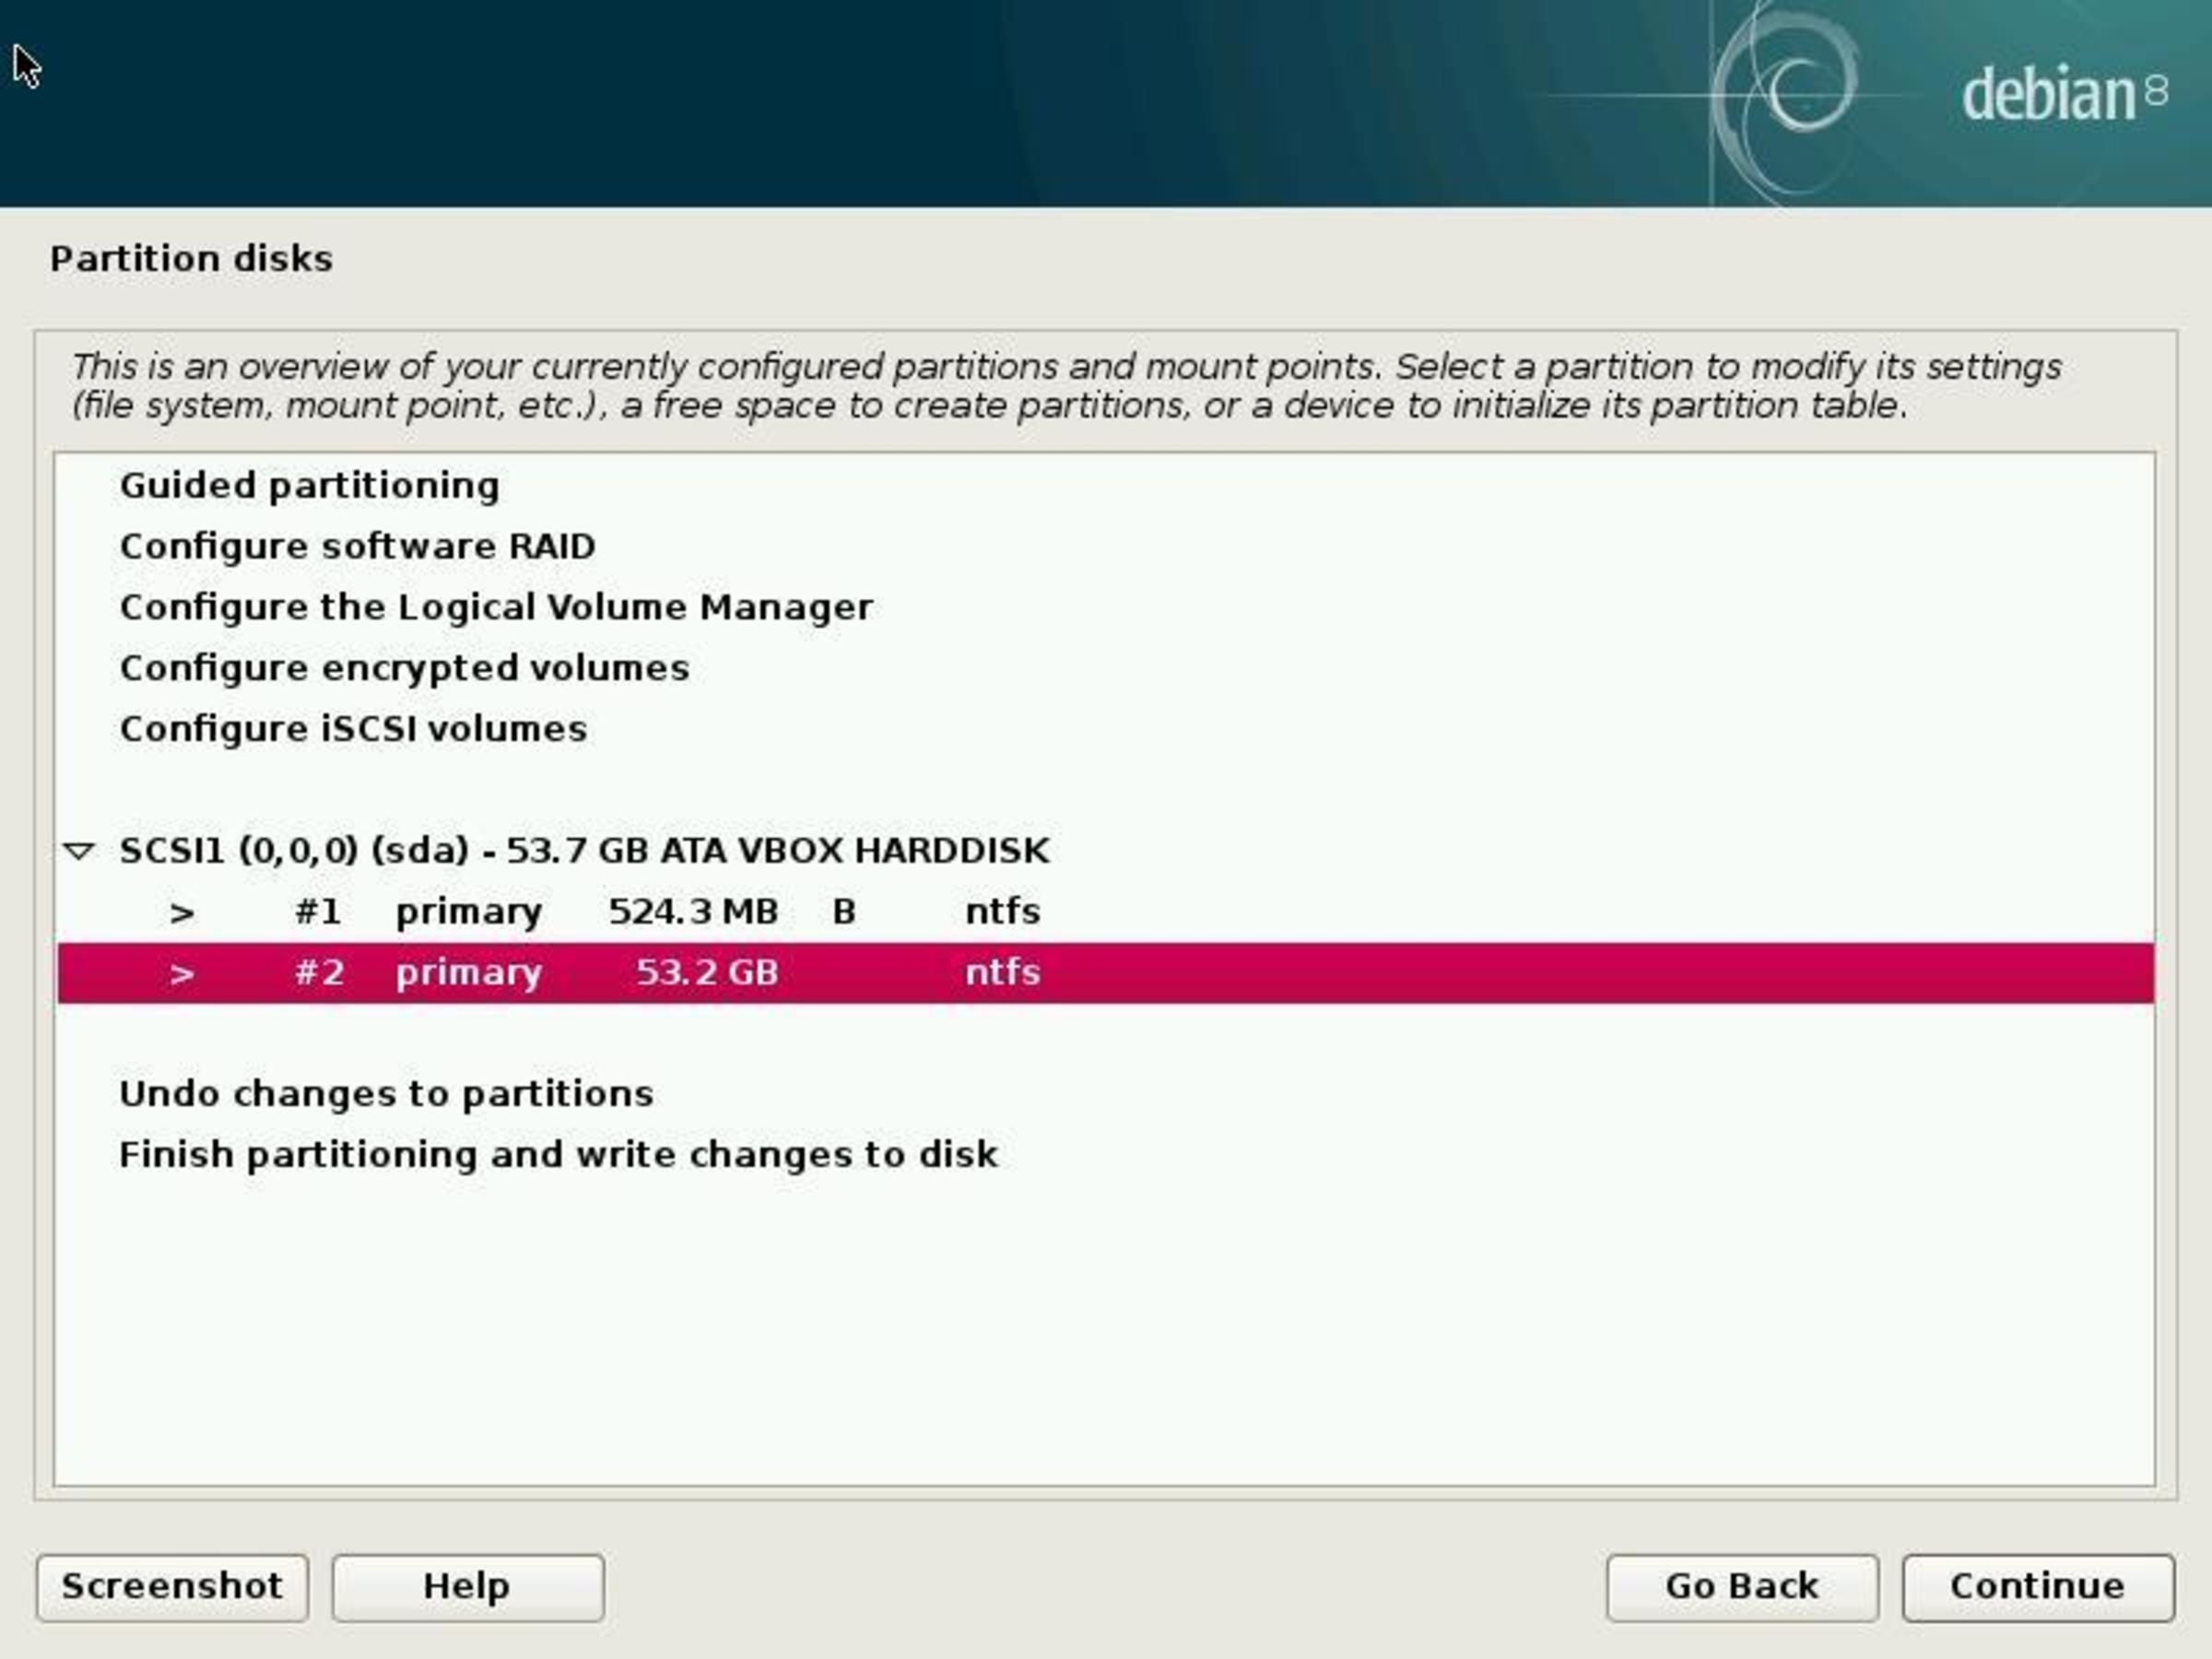
\includegraphics{resize-partition}
	\caption{Selezione della partizione di Windows da ridimensionare}
	\label{fig:resize-partition}
\end{figure}

Dopodiché Debian ci chiederà cosa fare con la partizione selezionata: scegliamo \texttt{Resize the partition} (\texttt{Ridimensionare la partizione}). Quindi ci verrà chiesto di salvare le modifiche fatte finora (anche se non abbiamo ancora fatto nessuna modifica, Debian ce lo chiede comunque): rispondiamo affermativamente con \texttt{Yes} (\texttt{Sì}). Infine, ci verrà chiesta la nuova dimensione per la partizione: consigliamo di riservare almeno \texttt{30 GB} per Debian, e quindi di ridurre la partizione di almeno \texttt{30 GB} rispetto alla dimensione originale.

Al termine ci ritroveremo nella lista delle partizioni: a questo punto dovrebbe essersi generata una quantità di spazio libero sufficiente a contenere Debian (Figura \vref{fig:select-free-space}).

%&pdflatex
\subsection{Partizioni per Debian}
Dobbiamo a questo punto selezionare lo spazio libero sul disco, come in Figura \vref{fig:select-free-space}.

\begin{figure}[ht]
	\centering
	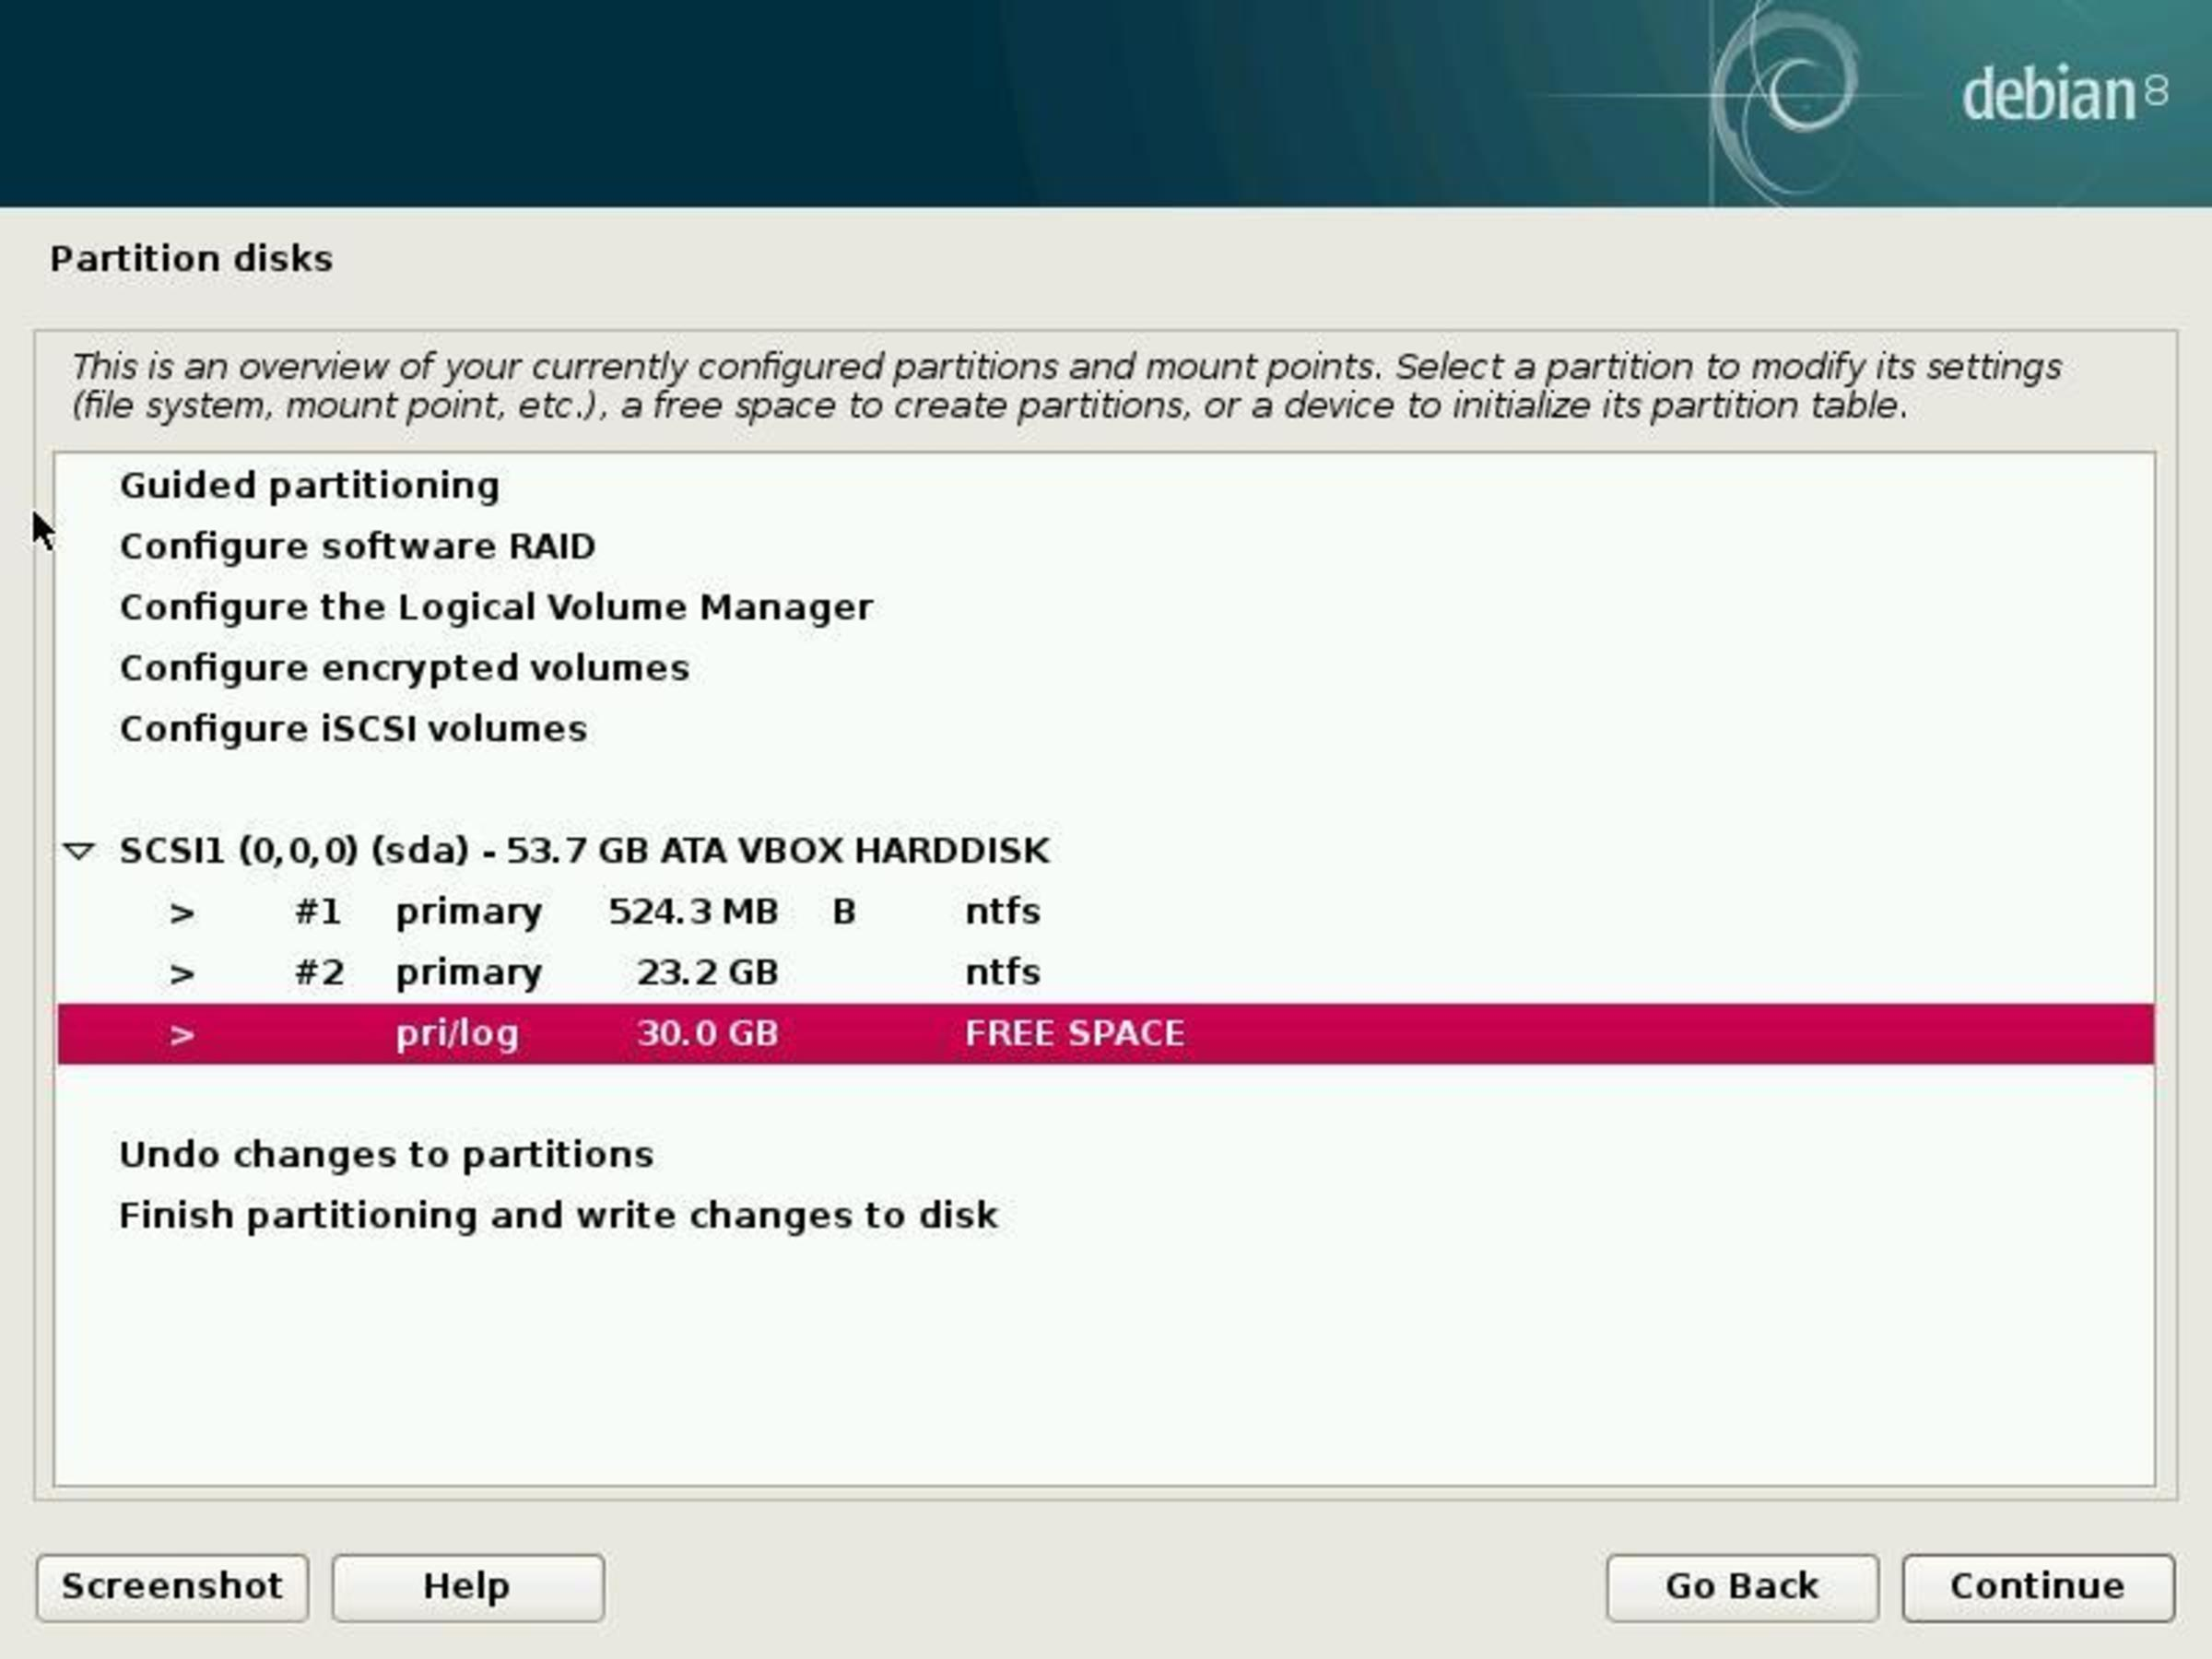
\includegraphics{select-free-space}
	\caption{Selezione dello spazio libero da utilizzare per le partizioni di Debian}
	\label{fig:select-free-space}
\end{figure}

Nella schermata successiva, selezioniamo \texttt{Automatically parti\-tion the free space} (\texttt{Partizionare automaticamente lo spa\-zio libero}). A questo punto saremo ricondotti al partizionamento guidato di Figura \vref{fig:partitioning}. Si scelga il partizionamento preferito (consigliamo di evitare di separare \texttt{/var} e \texttt{/tmp}).

\begin{figure}[ht]
	\centering
	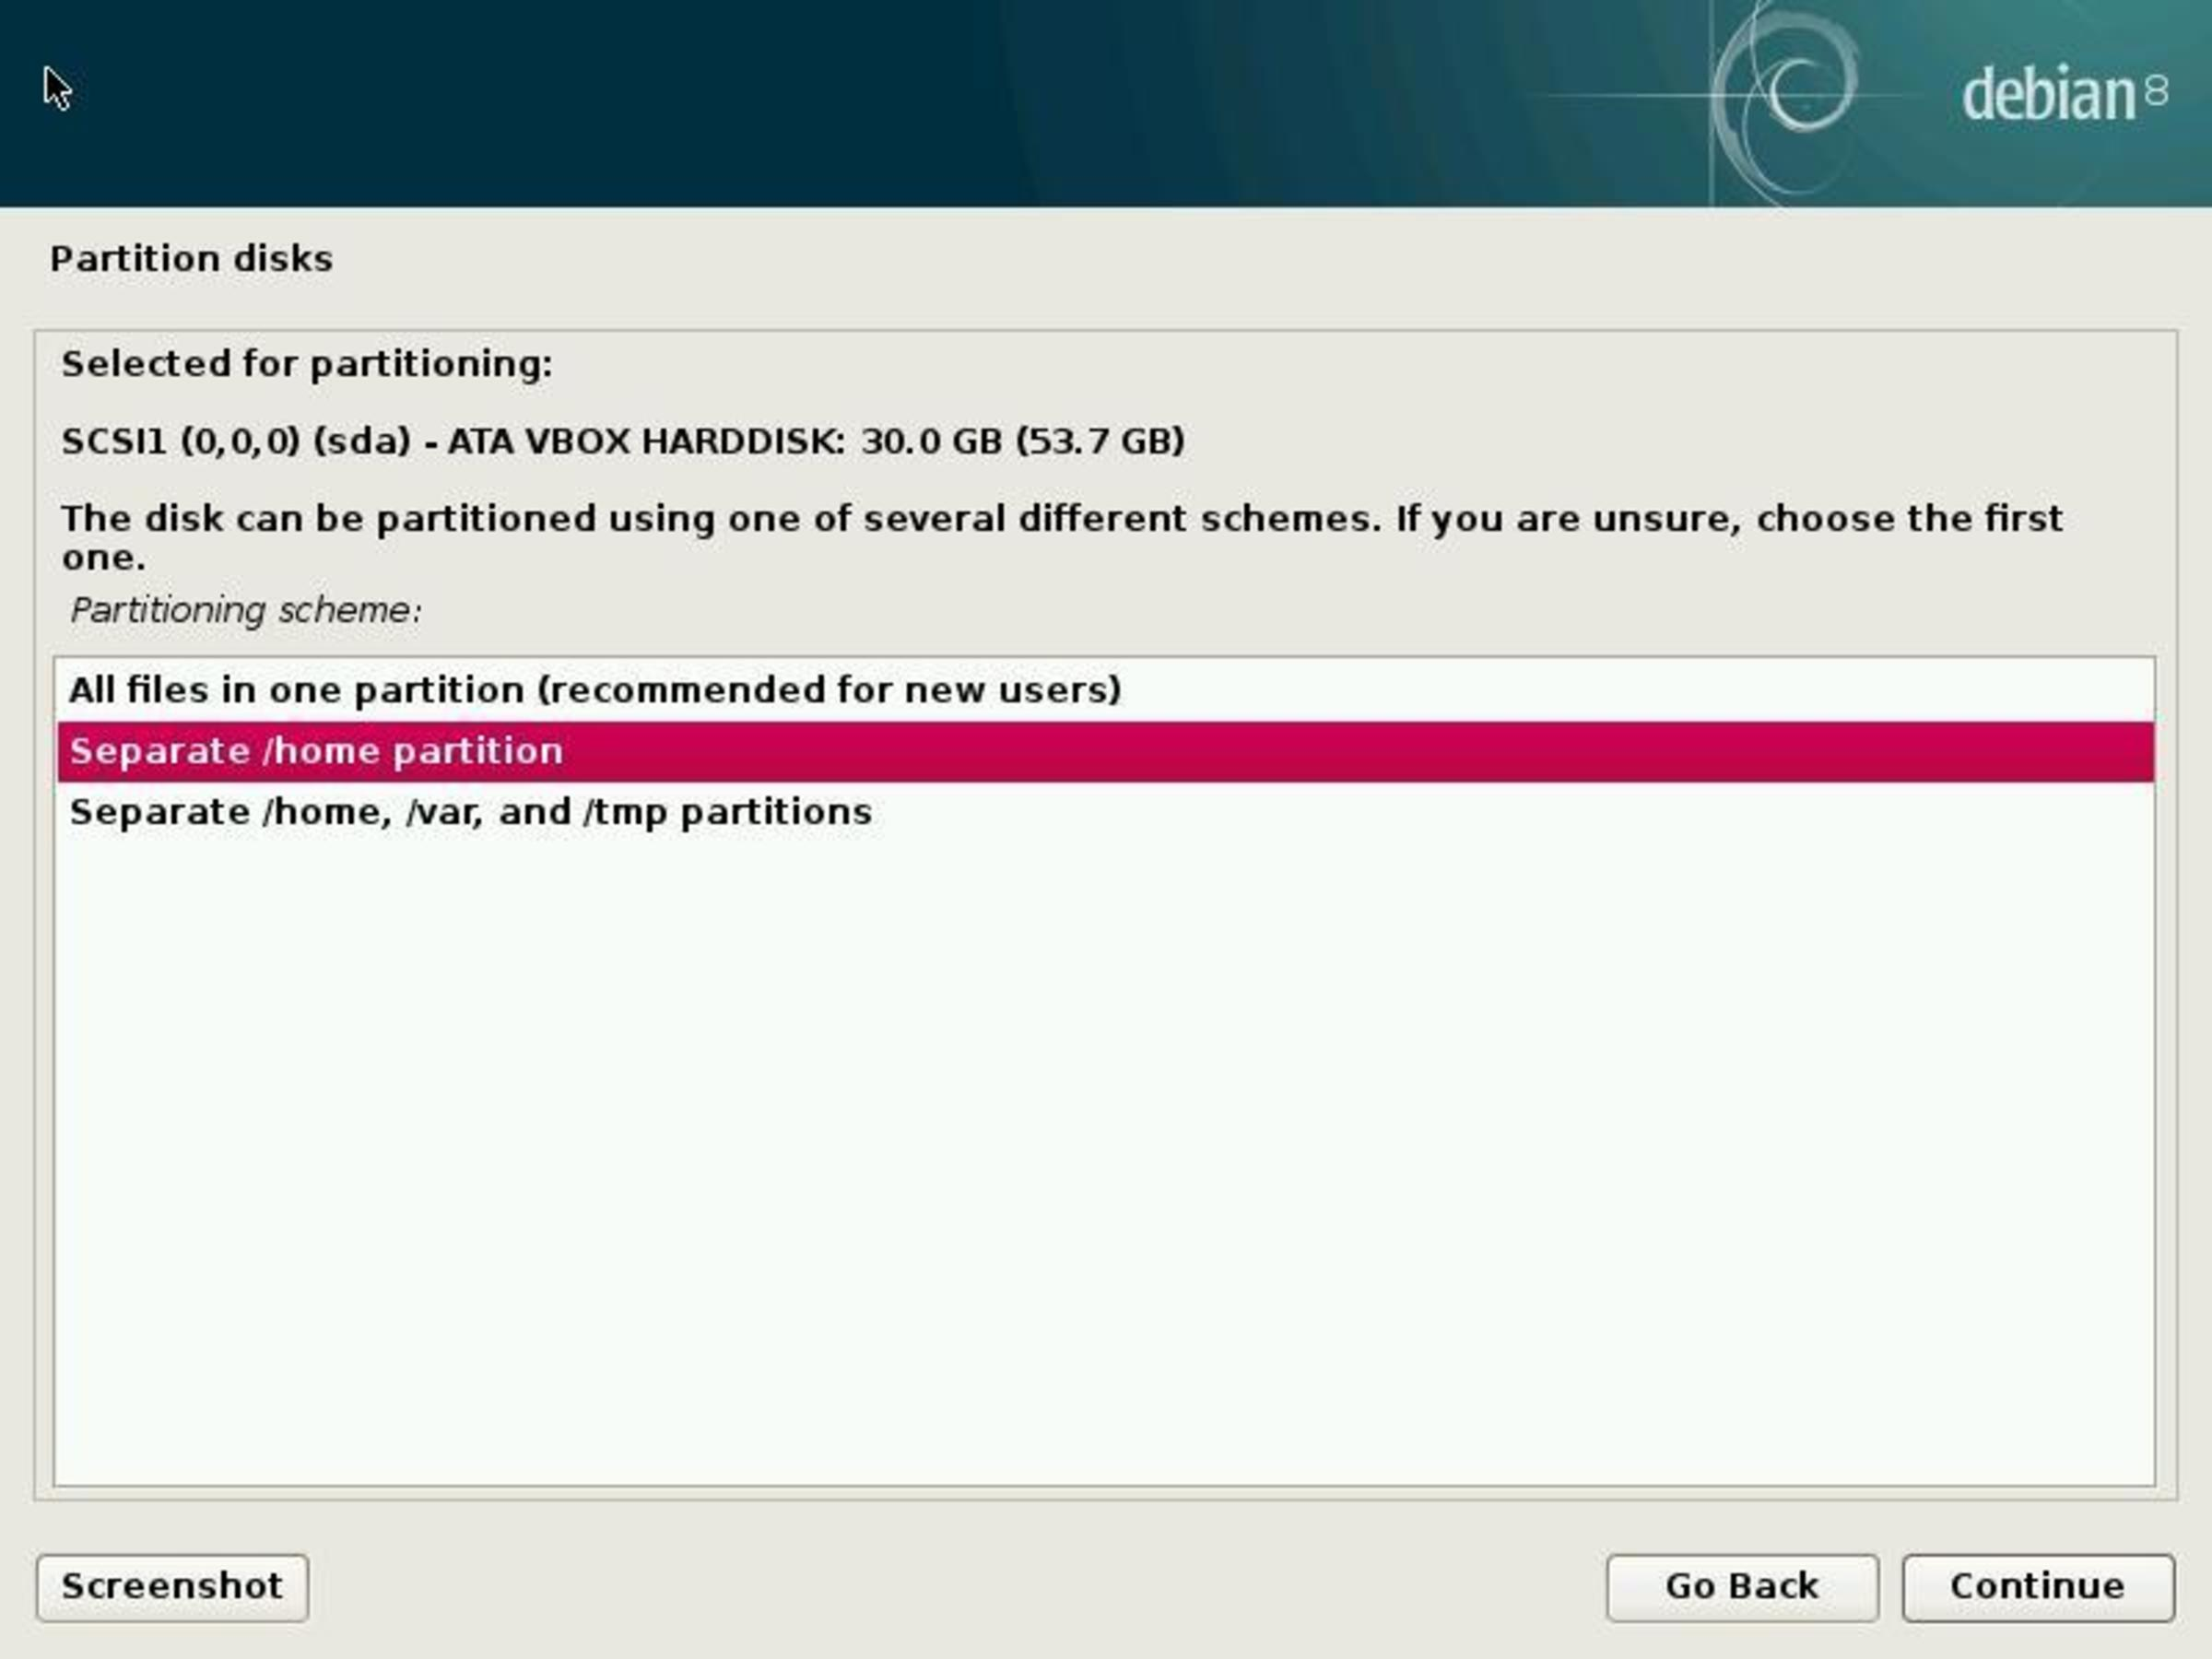
\includegraphics{partitioning}
	\caption{Selezione dello schema delle partizioni con partizionamento guidato}
	\label{fig:partitioning}
\end{figure}

A questo punto Debian ci farà vedere lo schema finale. Selezioniamo quindi \texttt{Finish partitioning and write changes to disk} (\texttt{Terminare il partizionamento e scrivere le modifiche sul disco}). Rispondiamo affermativamente alla domanda di conferma di scrittura delle modifiche su disco. Debian a questo punto salverà le nuove partizioni e inizierà ad installare il sistema di base.


%&pdflatex
\section{Configurazione del software}
Quando Debian avrà finito di installare il sistema di base, nella schermata successiva (Figura \vref{fig:apt-config}) ci verrà chiesto di configurare il \textit{package manager}. Come abbiamo già detto, il package manager è quel programma che serve ad installare le applicazioni. Debian, come package manager, usa \texttt{apt}.

\begin{figure}[ht]
	\centering
	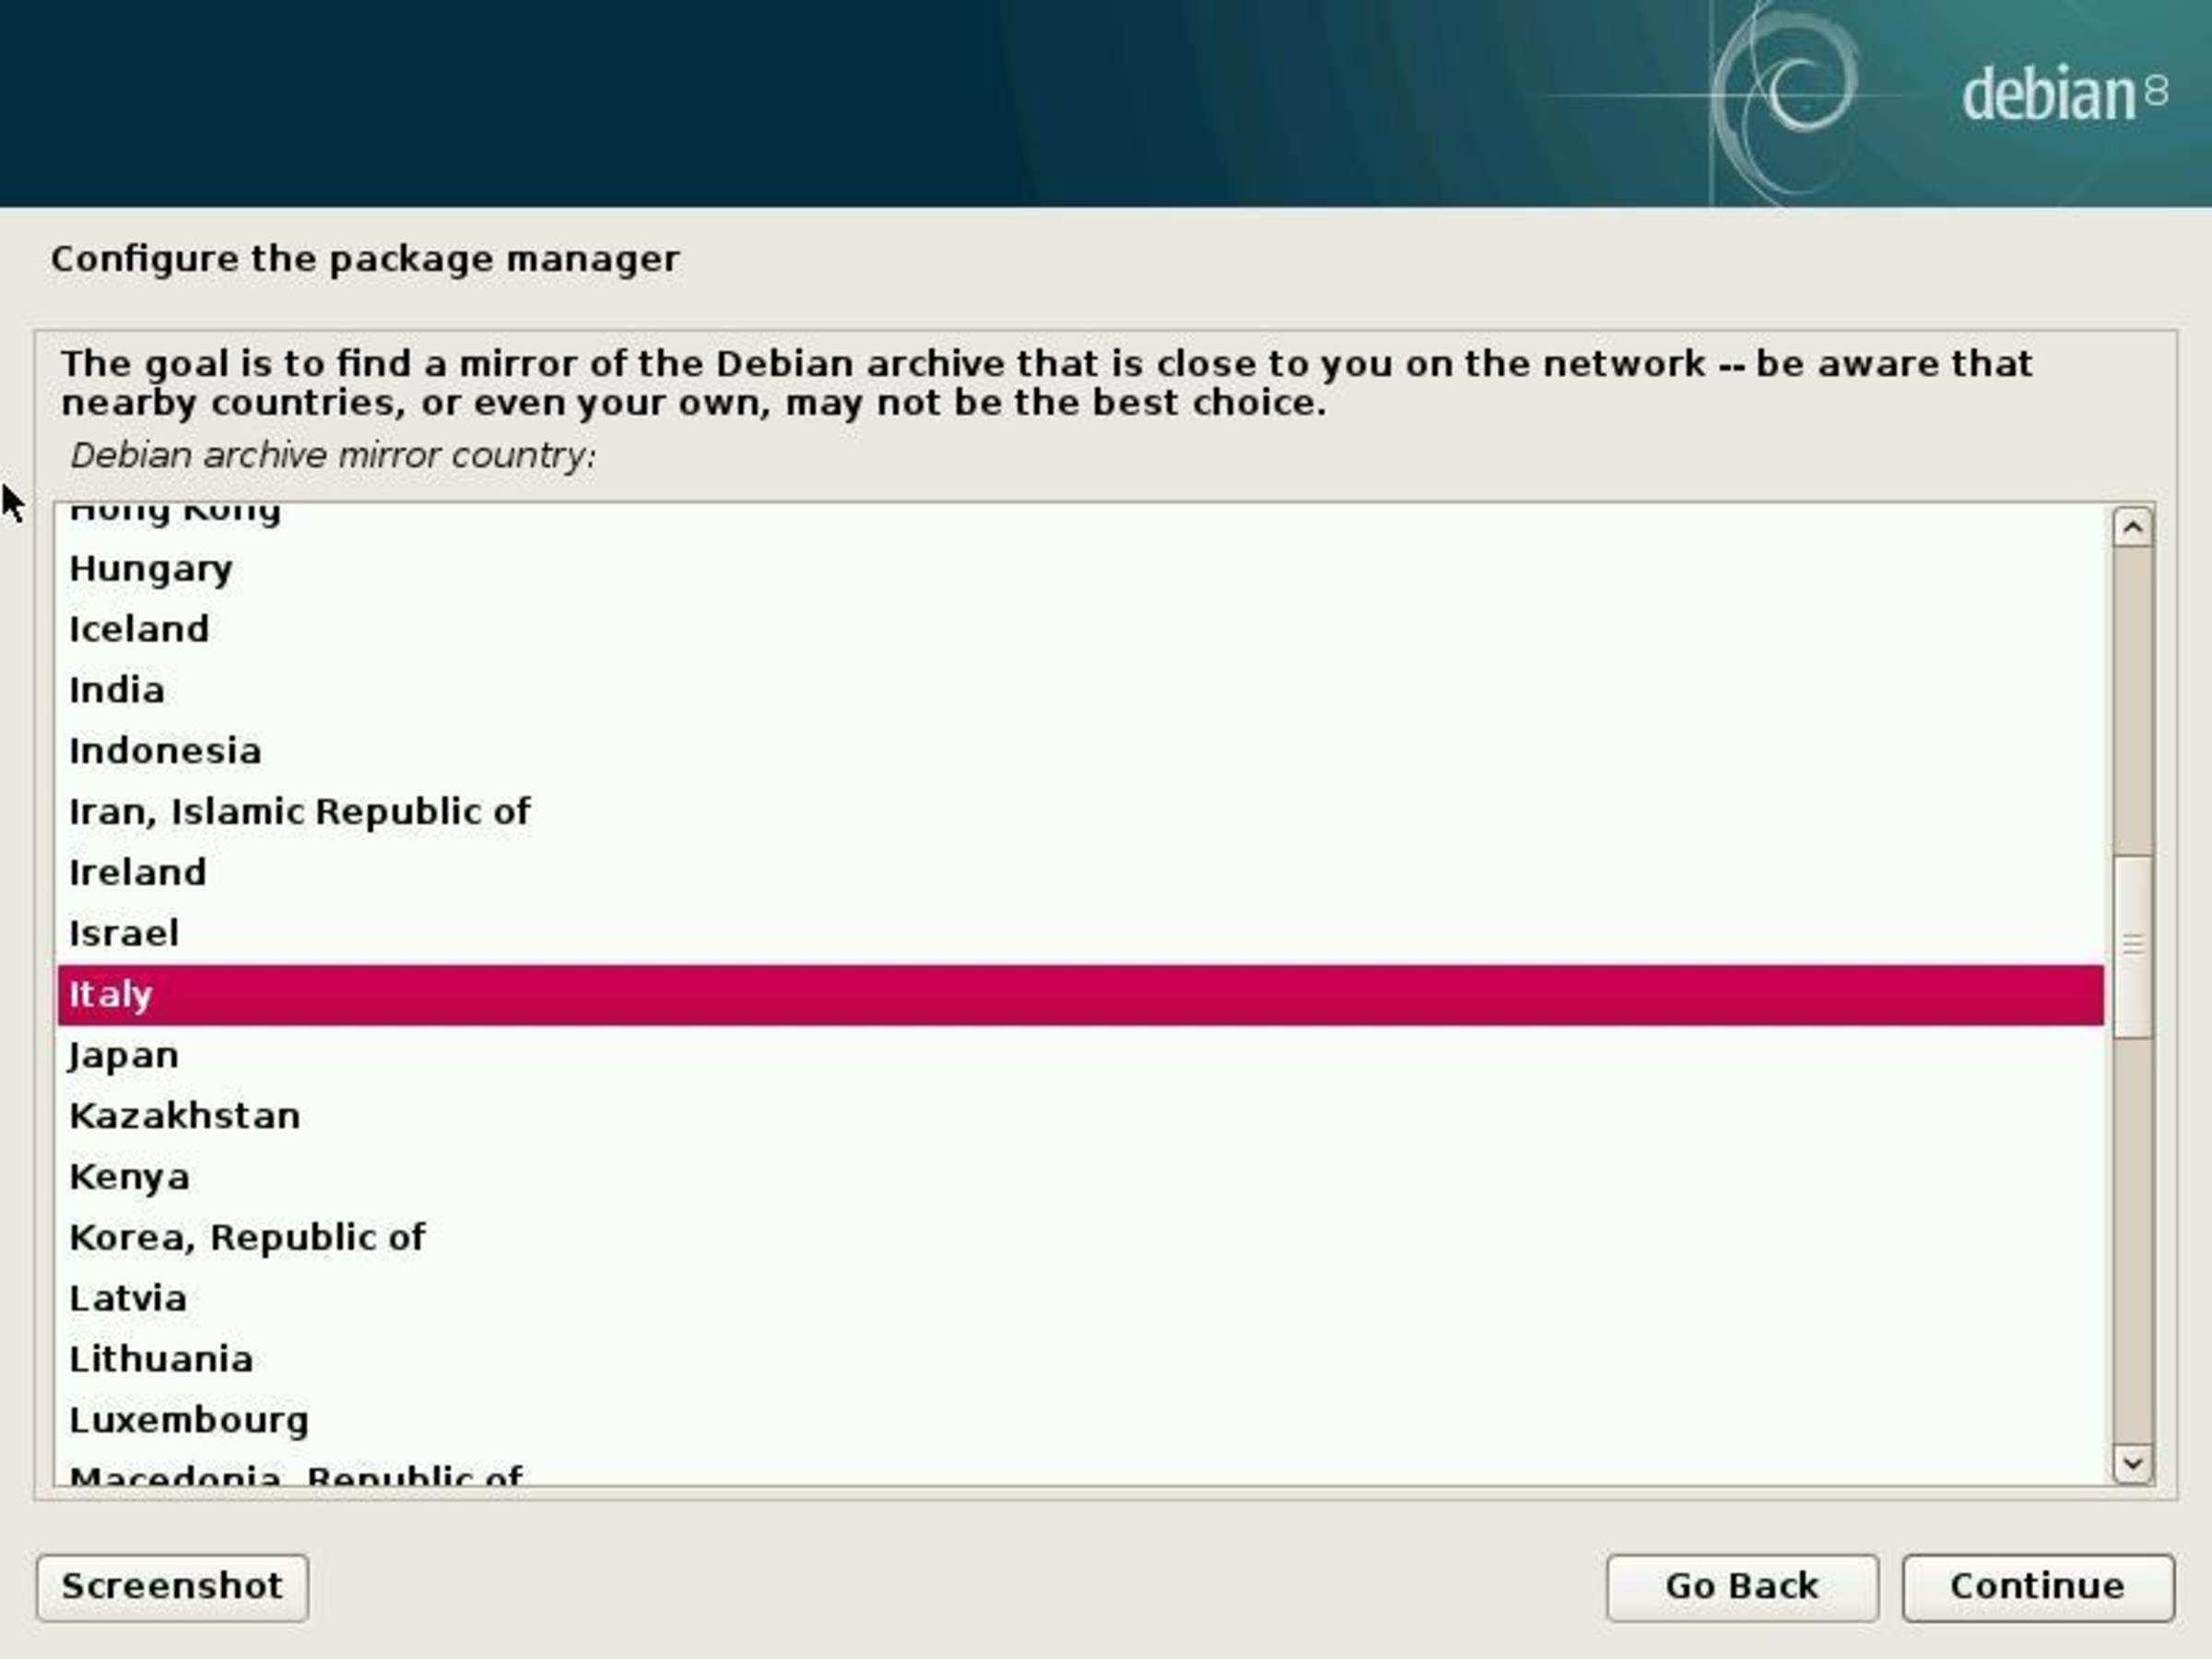
\includegraphics[resolution=600]{apt-config}
	\caption{Configurazione di \texttt{APT}: selezione del paese}
	\label{fig:apt-config}
\end{figure}

Selezioniamo \texttt{Italy} (\texttt{Italia}). Successivamente, ci verrà chiesto di scegliere il \textit{mirror} che si desidera utilizzare per scaricare il software. Tutti i mirror sono uguali, e dovrebbero funzionare ugualmente tutti quanti. Scegliamo \texttt{ftp.it.debian.org}.

Infine, viene chiesto se si desidera utilizzare un \textit{proxy HTTP}. Lasciamo il campo vuoto, ad indicare che non intendiamo utilizzare alcun proxy.

L'installer continuerà adesso ad installare altro software. Dopo un po', ci chiederà se vogliamo partecipare al \textit{popularity contest}, ossia alla raccolta dati anonima per determinare quali sono le applicazioni più utilizzate dagli utenti Debian nel mondo (Figura \vref{fig:popularity-contest}). Il lettore scelga ciò che preferisce.

\begin{figure}[ht]
	\centering
	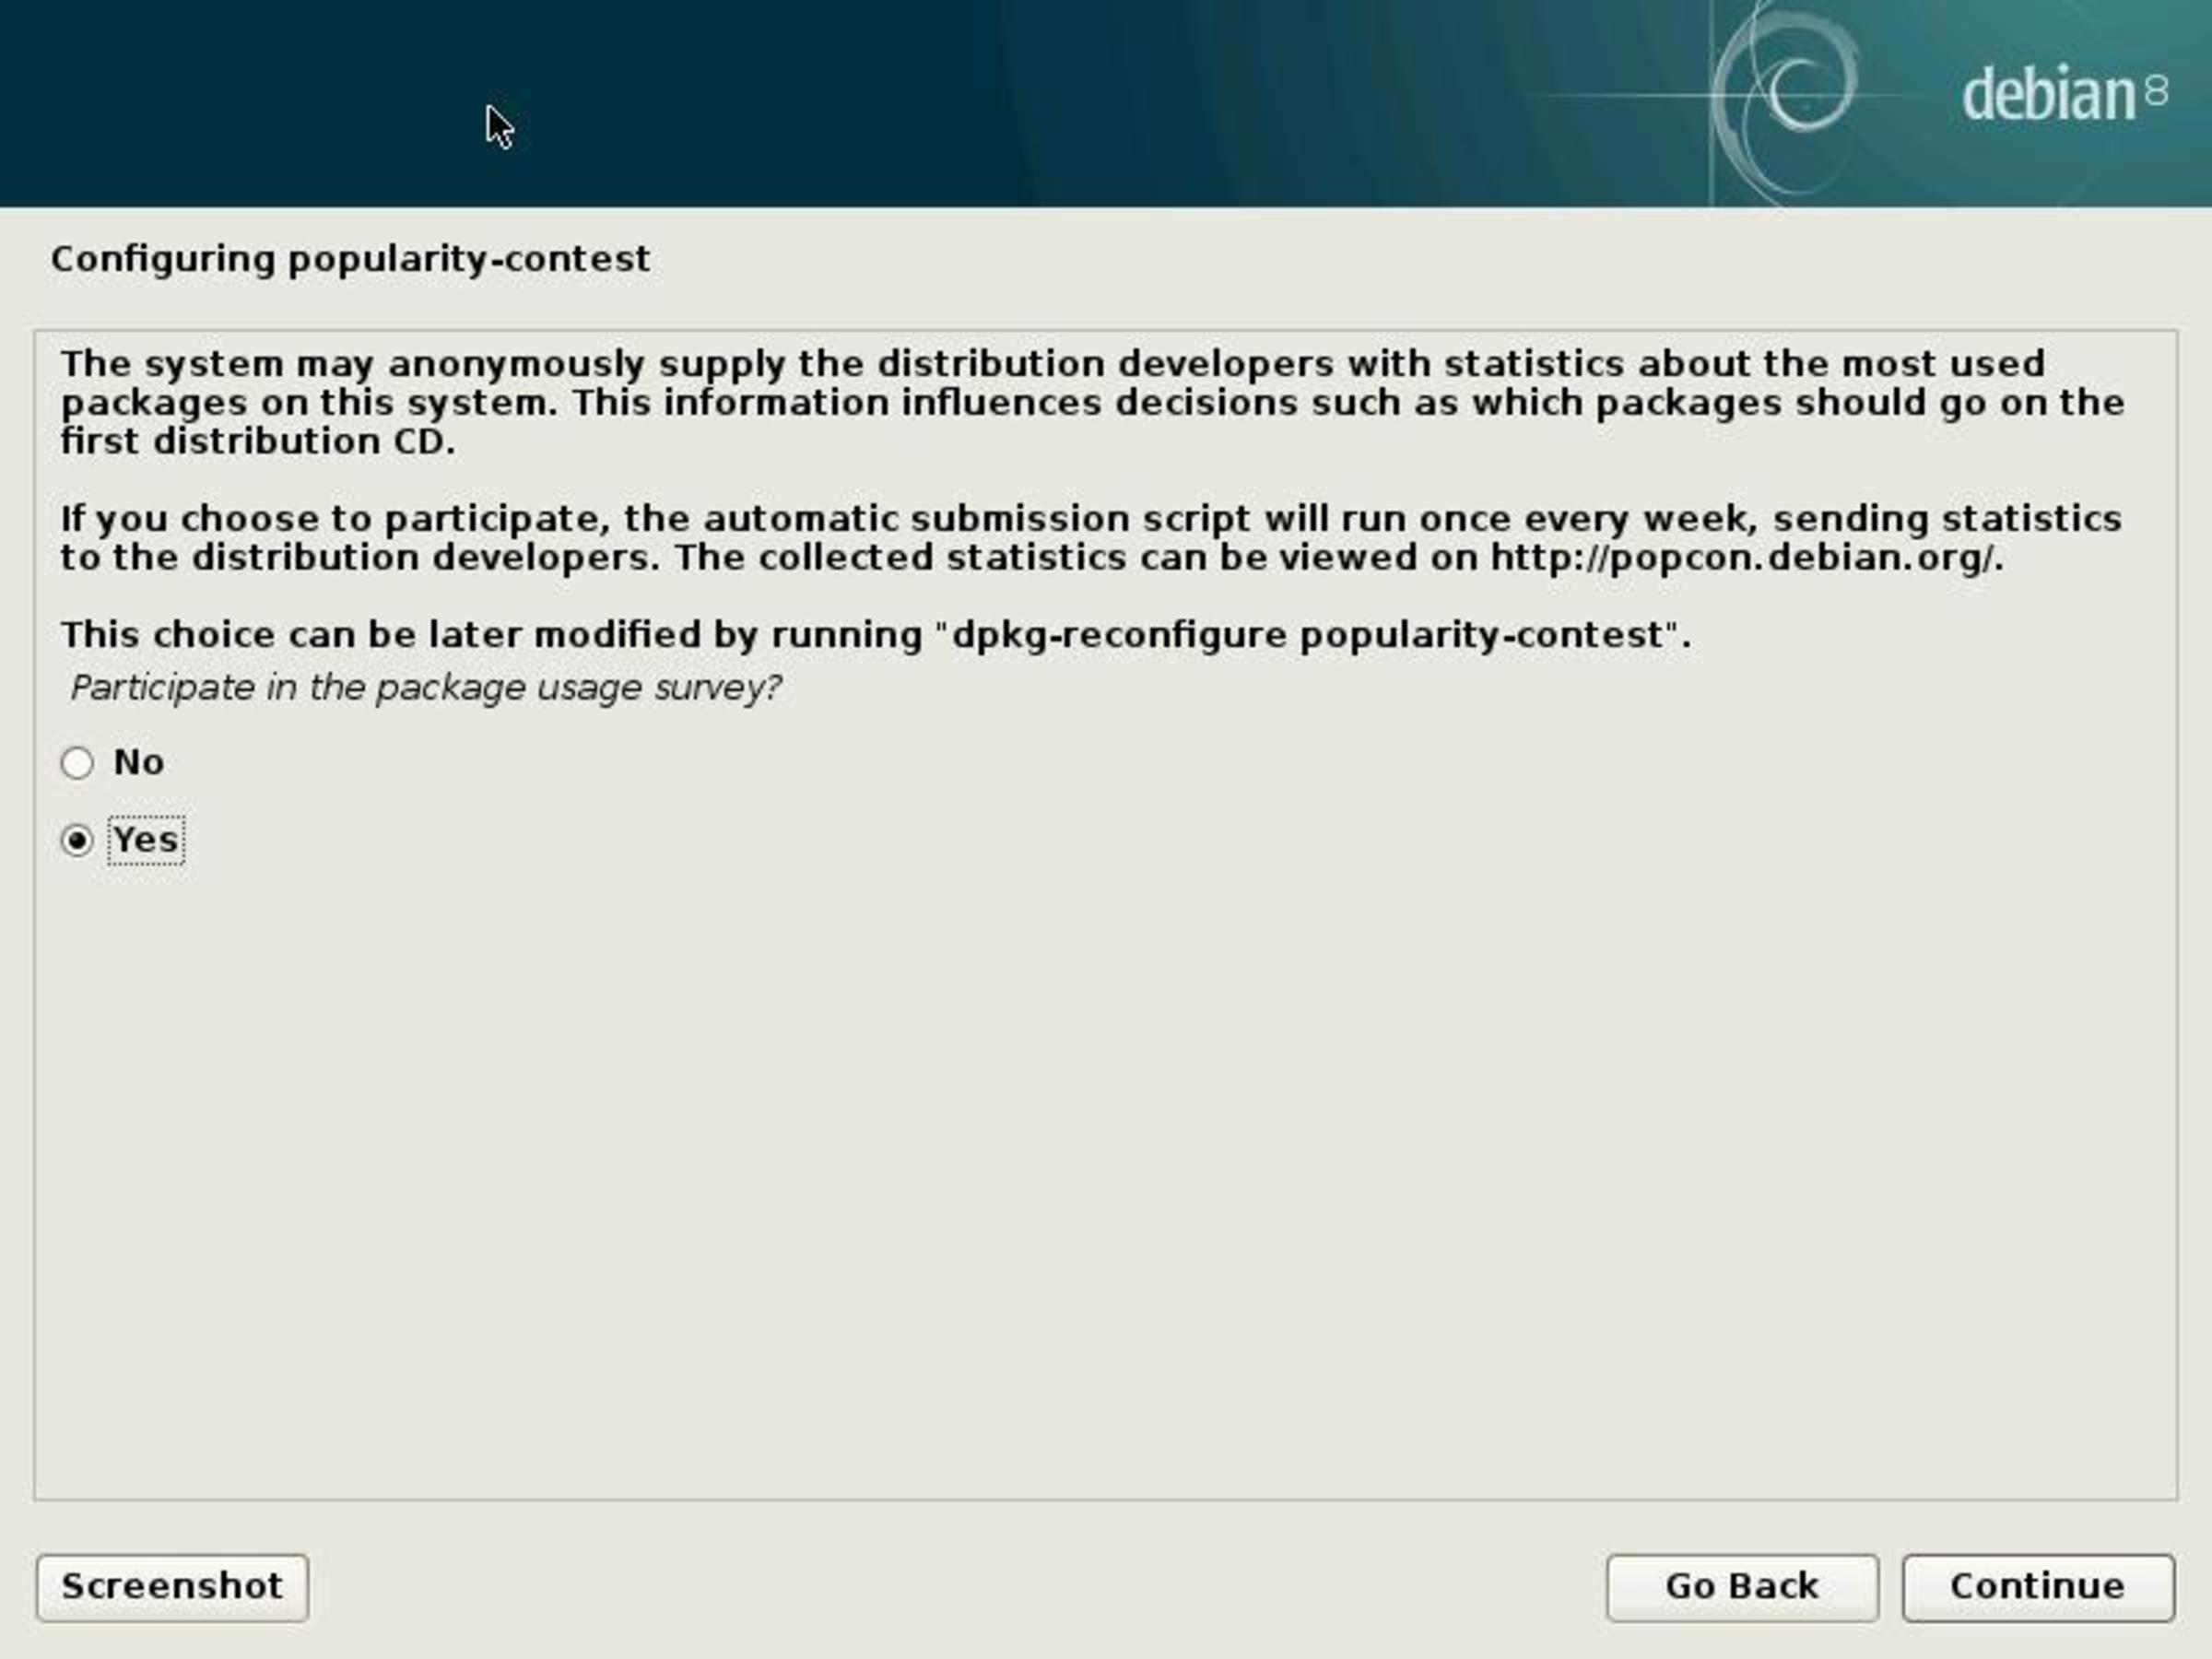
\includegraphics[resolution=600]{popularity-contest}
	\caption{Scelta di partecipazione al \textit{popularity contest}}
	\label{fig:popularity-contest}
\end{figure}


%&pdflatex
\section{Selezione del software}
L'ultimo passaggio riguarda l'installazione di software aggiuntivo su Debian. Possiamo scegliere se installare un \textit{desktop environment} (ambiente desktop) e quale installare; se vogliamo installare un \textit{web server}, un \textit{server di stampa} (\texttt{cups}), un \textit{server ssh} e le utility di base per l'amministrazione del sistema.

Il desktop environment è l'ambiente grafico. Se non scegliamo nessun desktop environment ci ritroveremo con un sistema operativo con la sola linea di comando (terminale) dove poter digitare comandi uno per volta. Per installare un desktop environment, dobbiamo selezionare la voce \texttt{Debian desktop environment} (\texttt{Ambiente desktop Debian}) e una (e una soltanto) delle voci sottostanti (\texttt{GNOME}, \texttt{Xfce}, \texttt{KDE}, \texttt{Cinnamon}, \texttt{MATE}, \texttt{LXDE}). La scelta, va fatta in base alle proprie preferenze. Di seguito, elenchiamo alcune caratteristiche di ognuno di questi desktop environment:
\begin{itemize}
	\item \textbf{GNOME} è il desktop environment più utilizzato al mondo. Ha come scopo l'usabilità e l'immediatezza d'uso, senza rinunciare all'estetica. Contiene molti programmi preinstallati;
	\item \textbf{Xfce} è un desktop environment minimale e leggero, adatto a chi preferisce un desktop environment essenziale e funzionale;
	\item \textbf{KDE} è un desktop environment molto potente e personalizzabile, ma anche molto pesante. Contiene molti programmi preinstallati;
	\item \textbf{Cinnamon} è il desktop environment prodotto dagli sviluppatori di \textit{Linux Mint}. Derivato di \texttt{GNOME}, è pensato per essere comodo e facile da usare;
	\item \textbf{MATE} è un desktop environment derivato dal codice di \texttt{GNOME 2} non più mantenuto dopo il rilascio della versione 3. È nato nel 2011 per iniziativa di alcuni membri della comunità di \textit{Arch Linux};
	\item \textbf{LXDE} Ambiente desktop minimale e veloce, ma con una grafica più accattivante di Xfce. Non è però più mantenuto, in quanto è stato rimpiazzato da \texttt{LXQT}.
\end{itemize}
Si consiglia al lettore di cercare con il proprio motore di ricerca preferito immagini riguardo ad ognuno di questi ambienti: può, in questo modo, farsi un'idea dell'aspetto grafico di questi desktop environment.

Il \textit{web server} non ci serve: è utile solo se vogliamo installare Debian su un server che dovrà ospitare un sito web. Non ci serve neanche il \textit{server SSH} che viene utilizzato per l'accesso remoto al sistema. Il \textit{print server} (server di stampa) è utile se vogliamo poter stampare documenti con una stampante da Debian. Infine, è consigliato installare le utility di sistema che servono a configurare e gestire al meglio il proprio ambiente.

Una possibile configurazione, dove viene installato Xfce come desktop environment, è quella mostrata in Figura \vref{fig:software-selection}. Dopo aver fatto avanti, l'installer inizierà a scaricare il software che abbiamo selezionato.

\begin{figure}[ht]
	\centering
	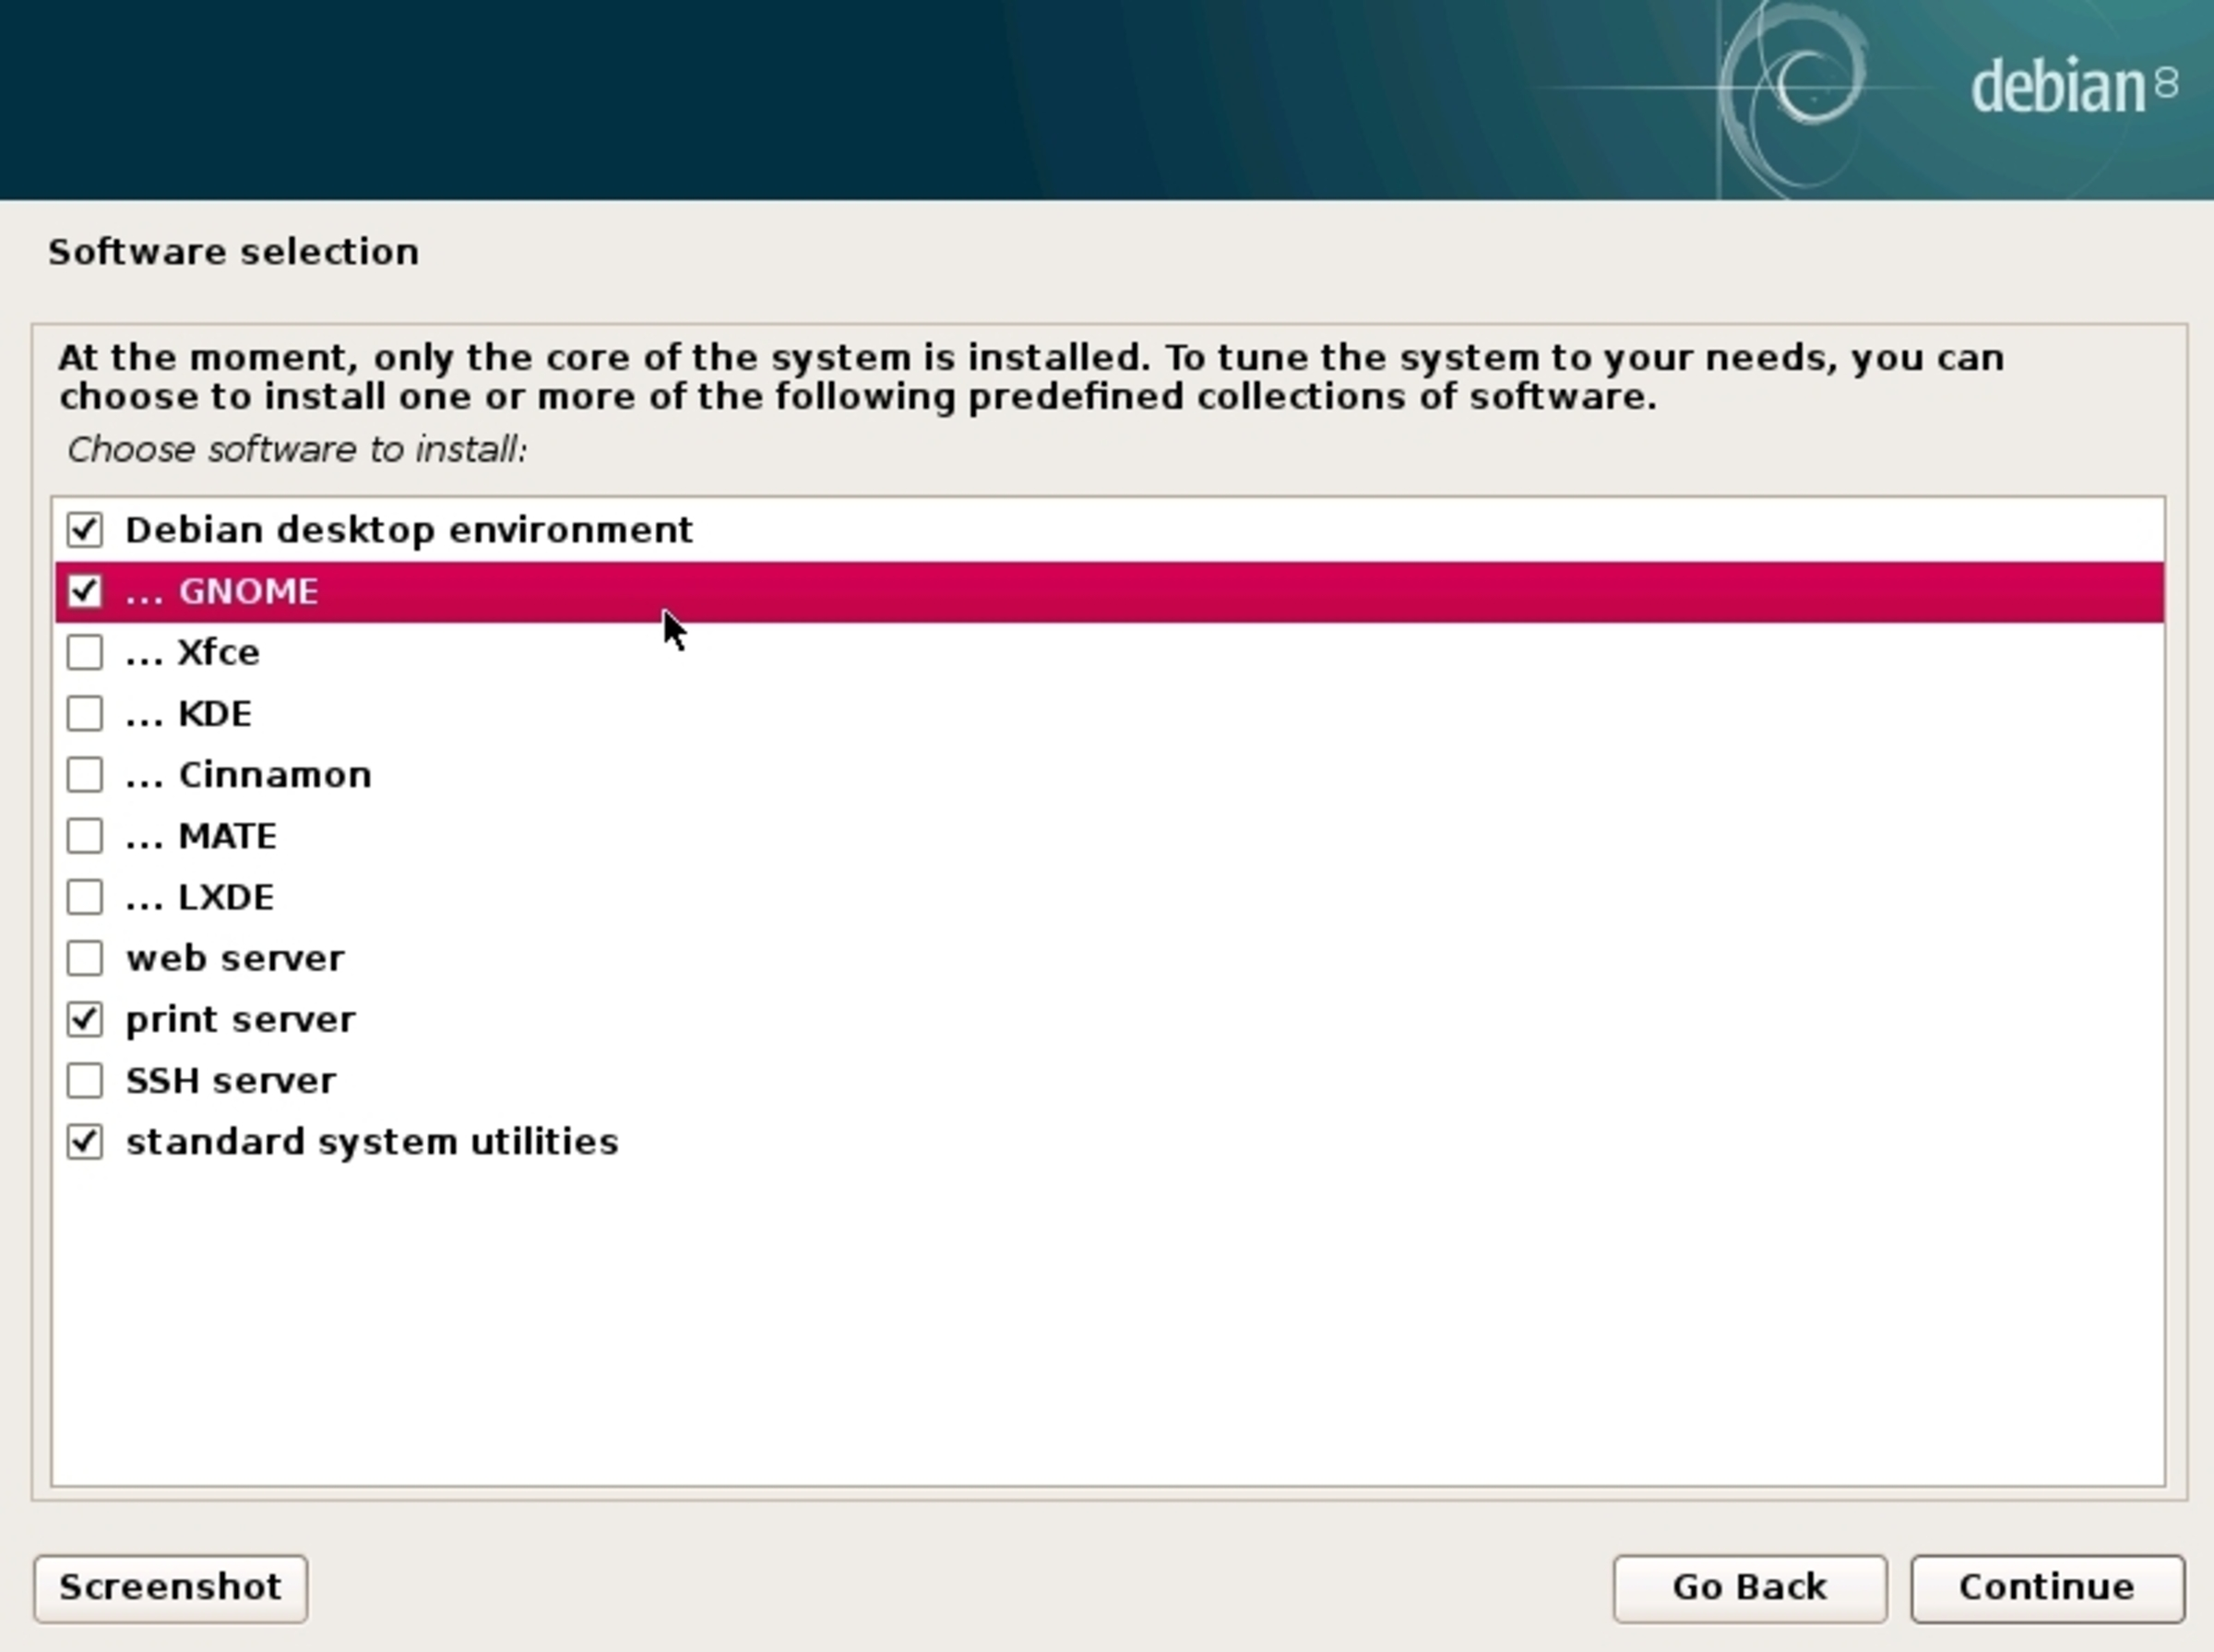
\includegraphics[resolution=600]{software-selection}
	\caption{Scelta del software e di Xfce come desktop environment}
	\label{fig:software-selection}
\end{figure}

%&pdflatex
\section{Bootloader e primo avvio}
L'ultimo passo è l'installazione del \textit{bootloader} (\texttt{GRUB}).

Senza un bootloader, Debian non potrebbe avviarsi. Quindi consigliamo di installare \texttt{GRUB} (bisogna rispondere \texttt{Yes} (\texttt{Sì}) alla domanda mostrata in Figura \vref{fig:install-grub}).

\begin{figure}[ht]
	\centering
	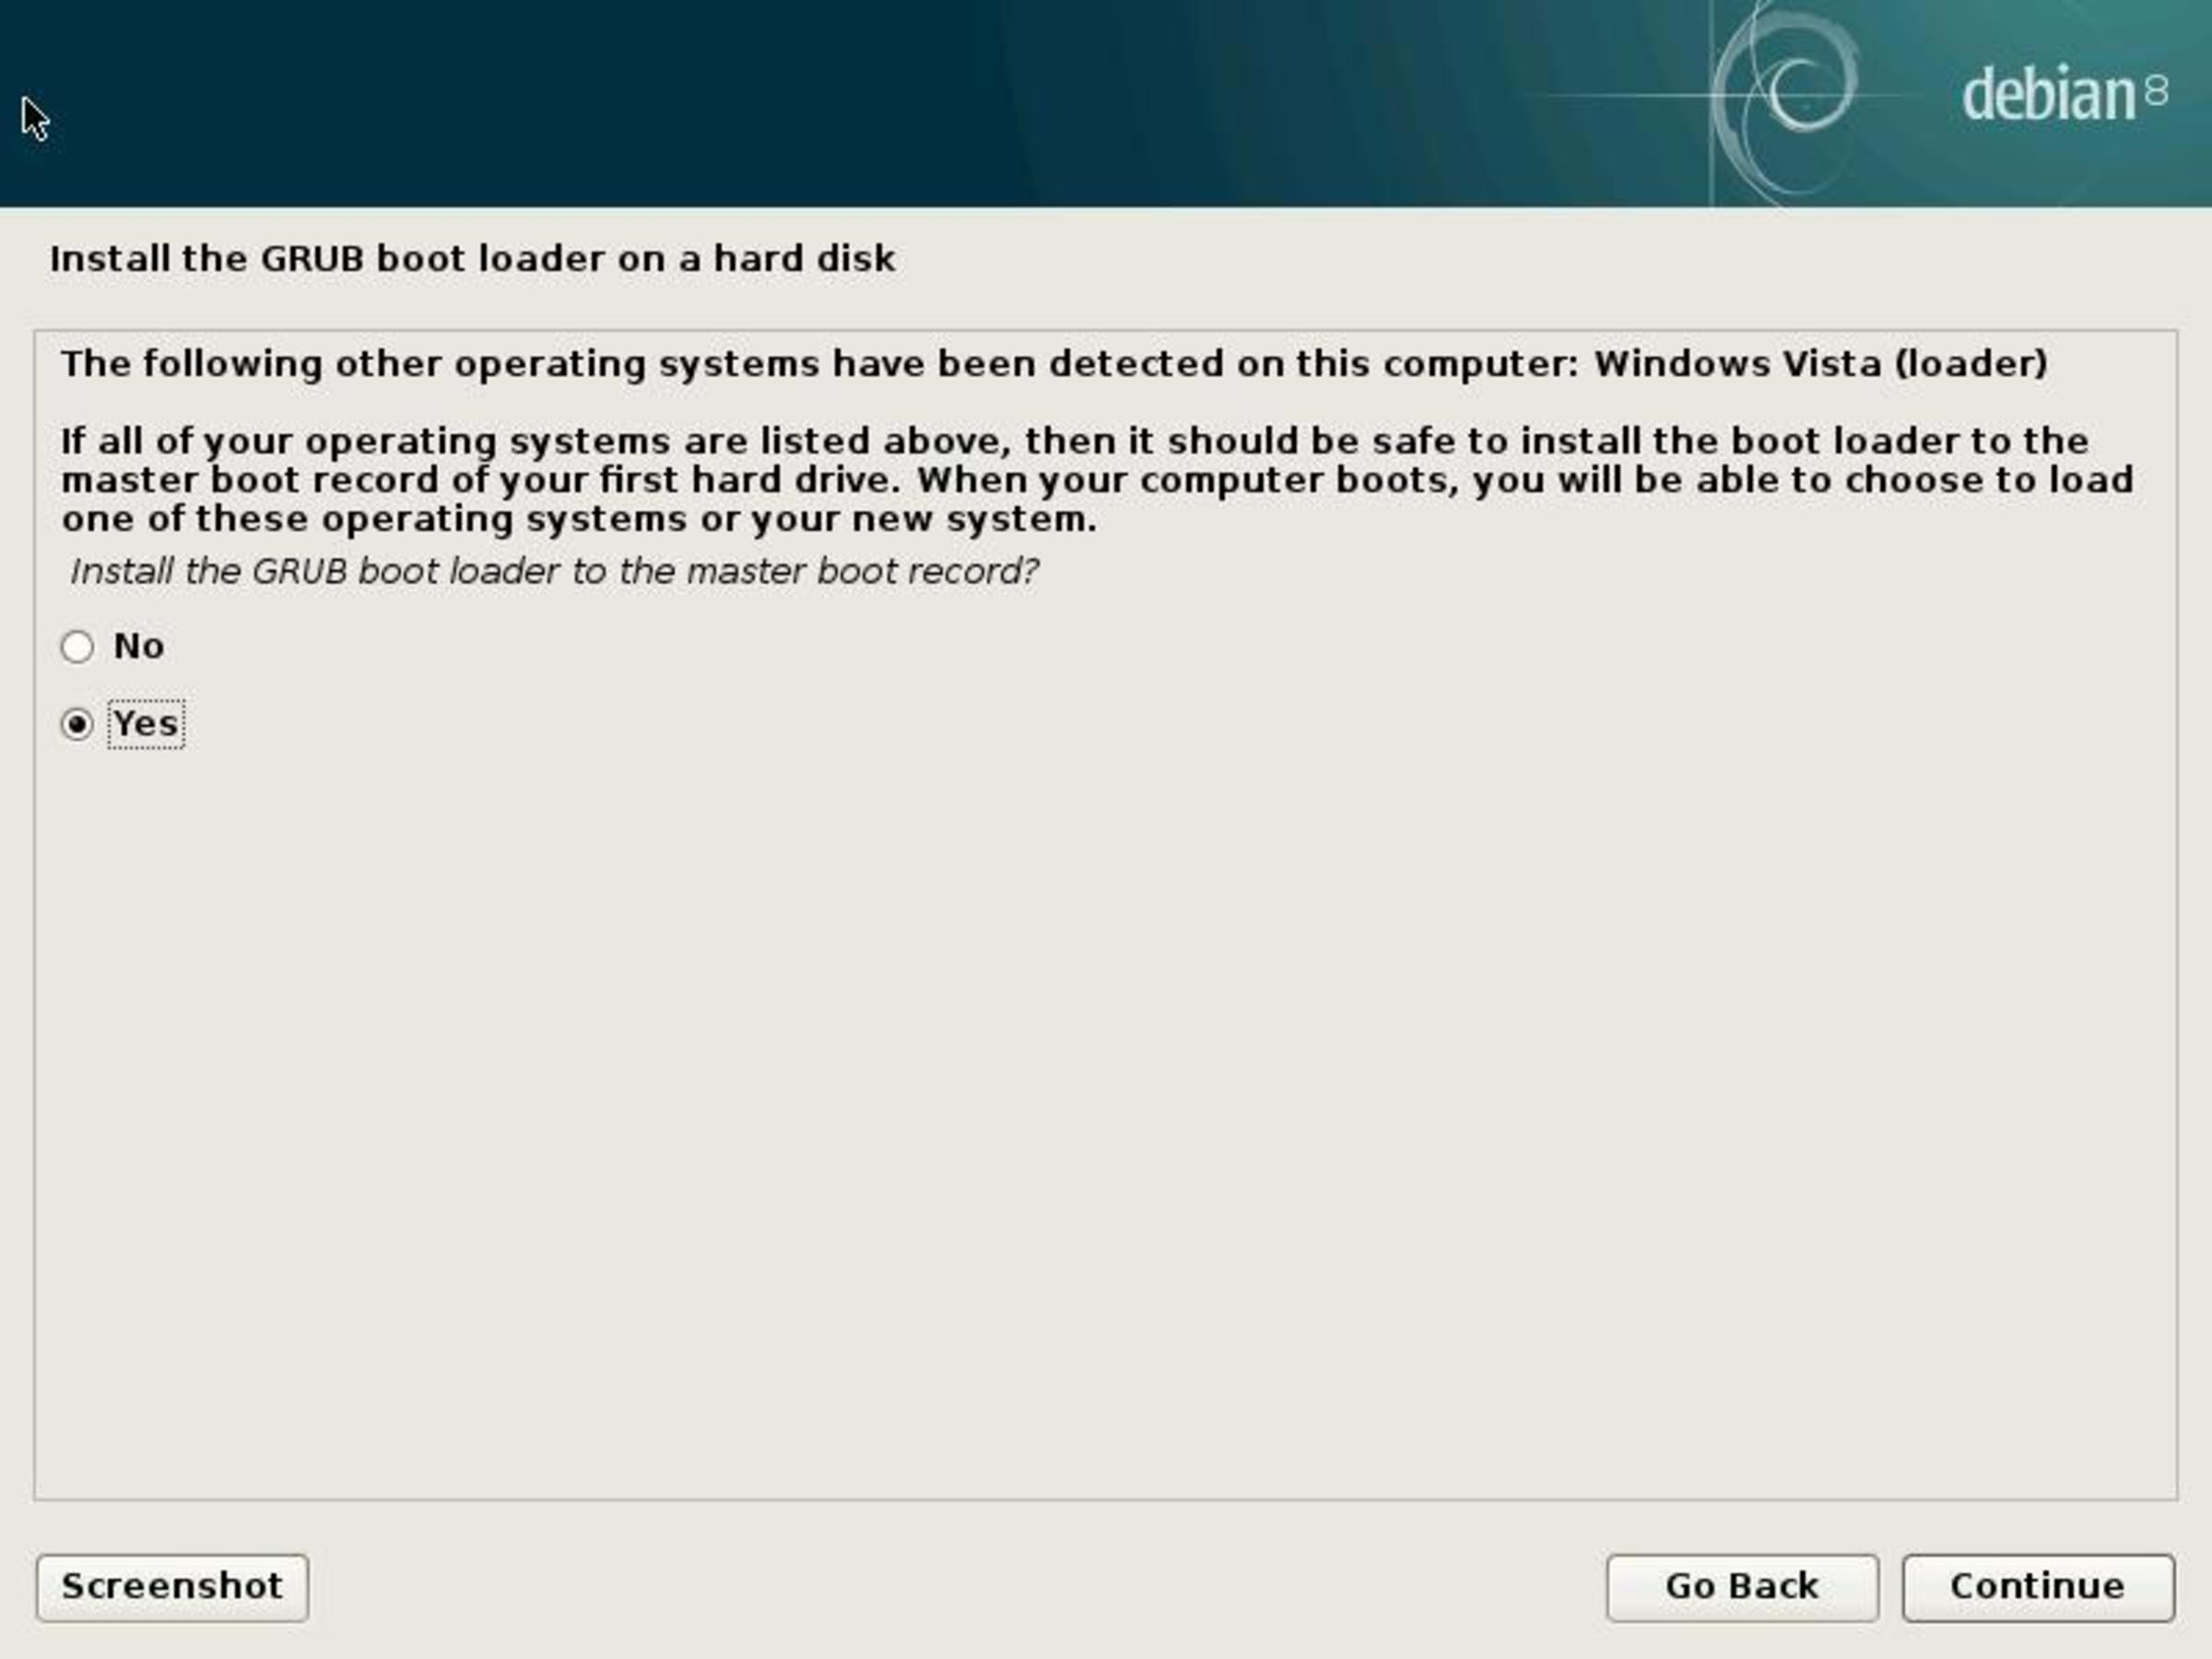
\includegraphics[resolution=600]{install-grub}
	\caption{Installazione di \texttt{GRUB}}
	\label{fig:install-grub}
\end{figure}

Nella schermata successiva, dobbiamo scegliere il disco sul quale si desidera installare \texttt{GRUB}. Si scelga il disco più adatto (di solito, lo stesso su cui si è installato Debian).

Infine, Debian ci chiede di rimuovere il disco di installazione del sistema. Rimuoviamo il disco (o il pendrive USB) e riavviamo cliccando su \texttt{Continue} (\texttt{Continua}).

Al riavvio, se tutto è andato per il meglio, dovrebbe comparire la schermata di \texttt{GRUB} mostrata in Figura \vref{fig:grub}.

\begin{figure}[ht]
	\centering
	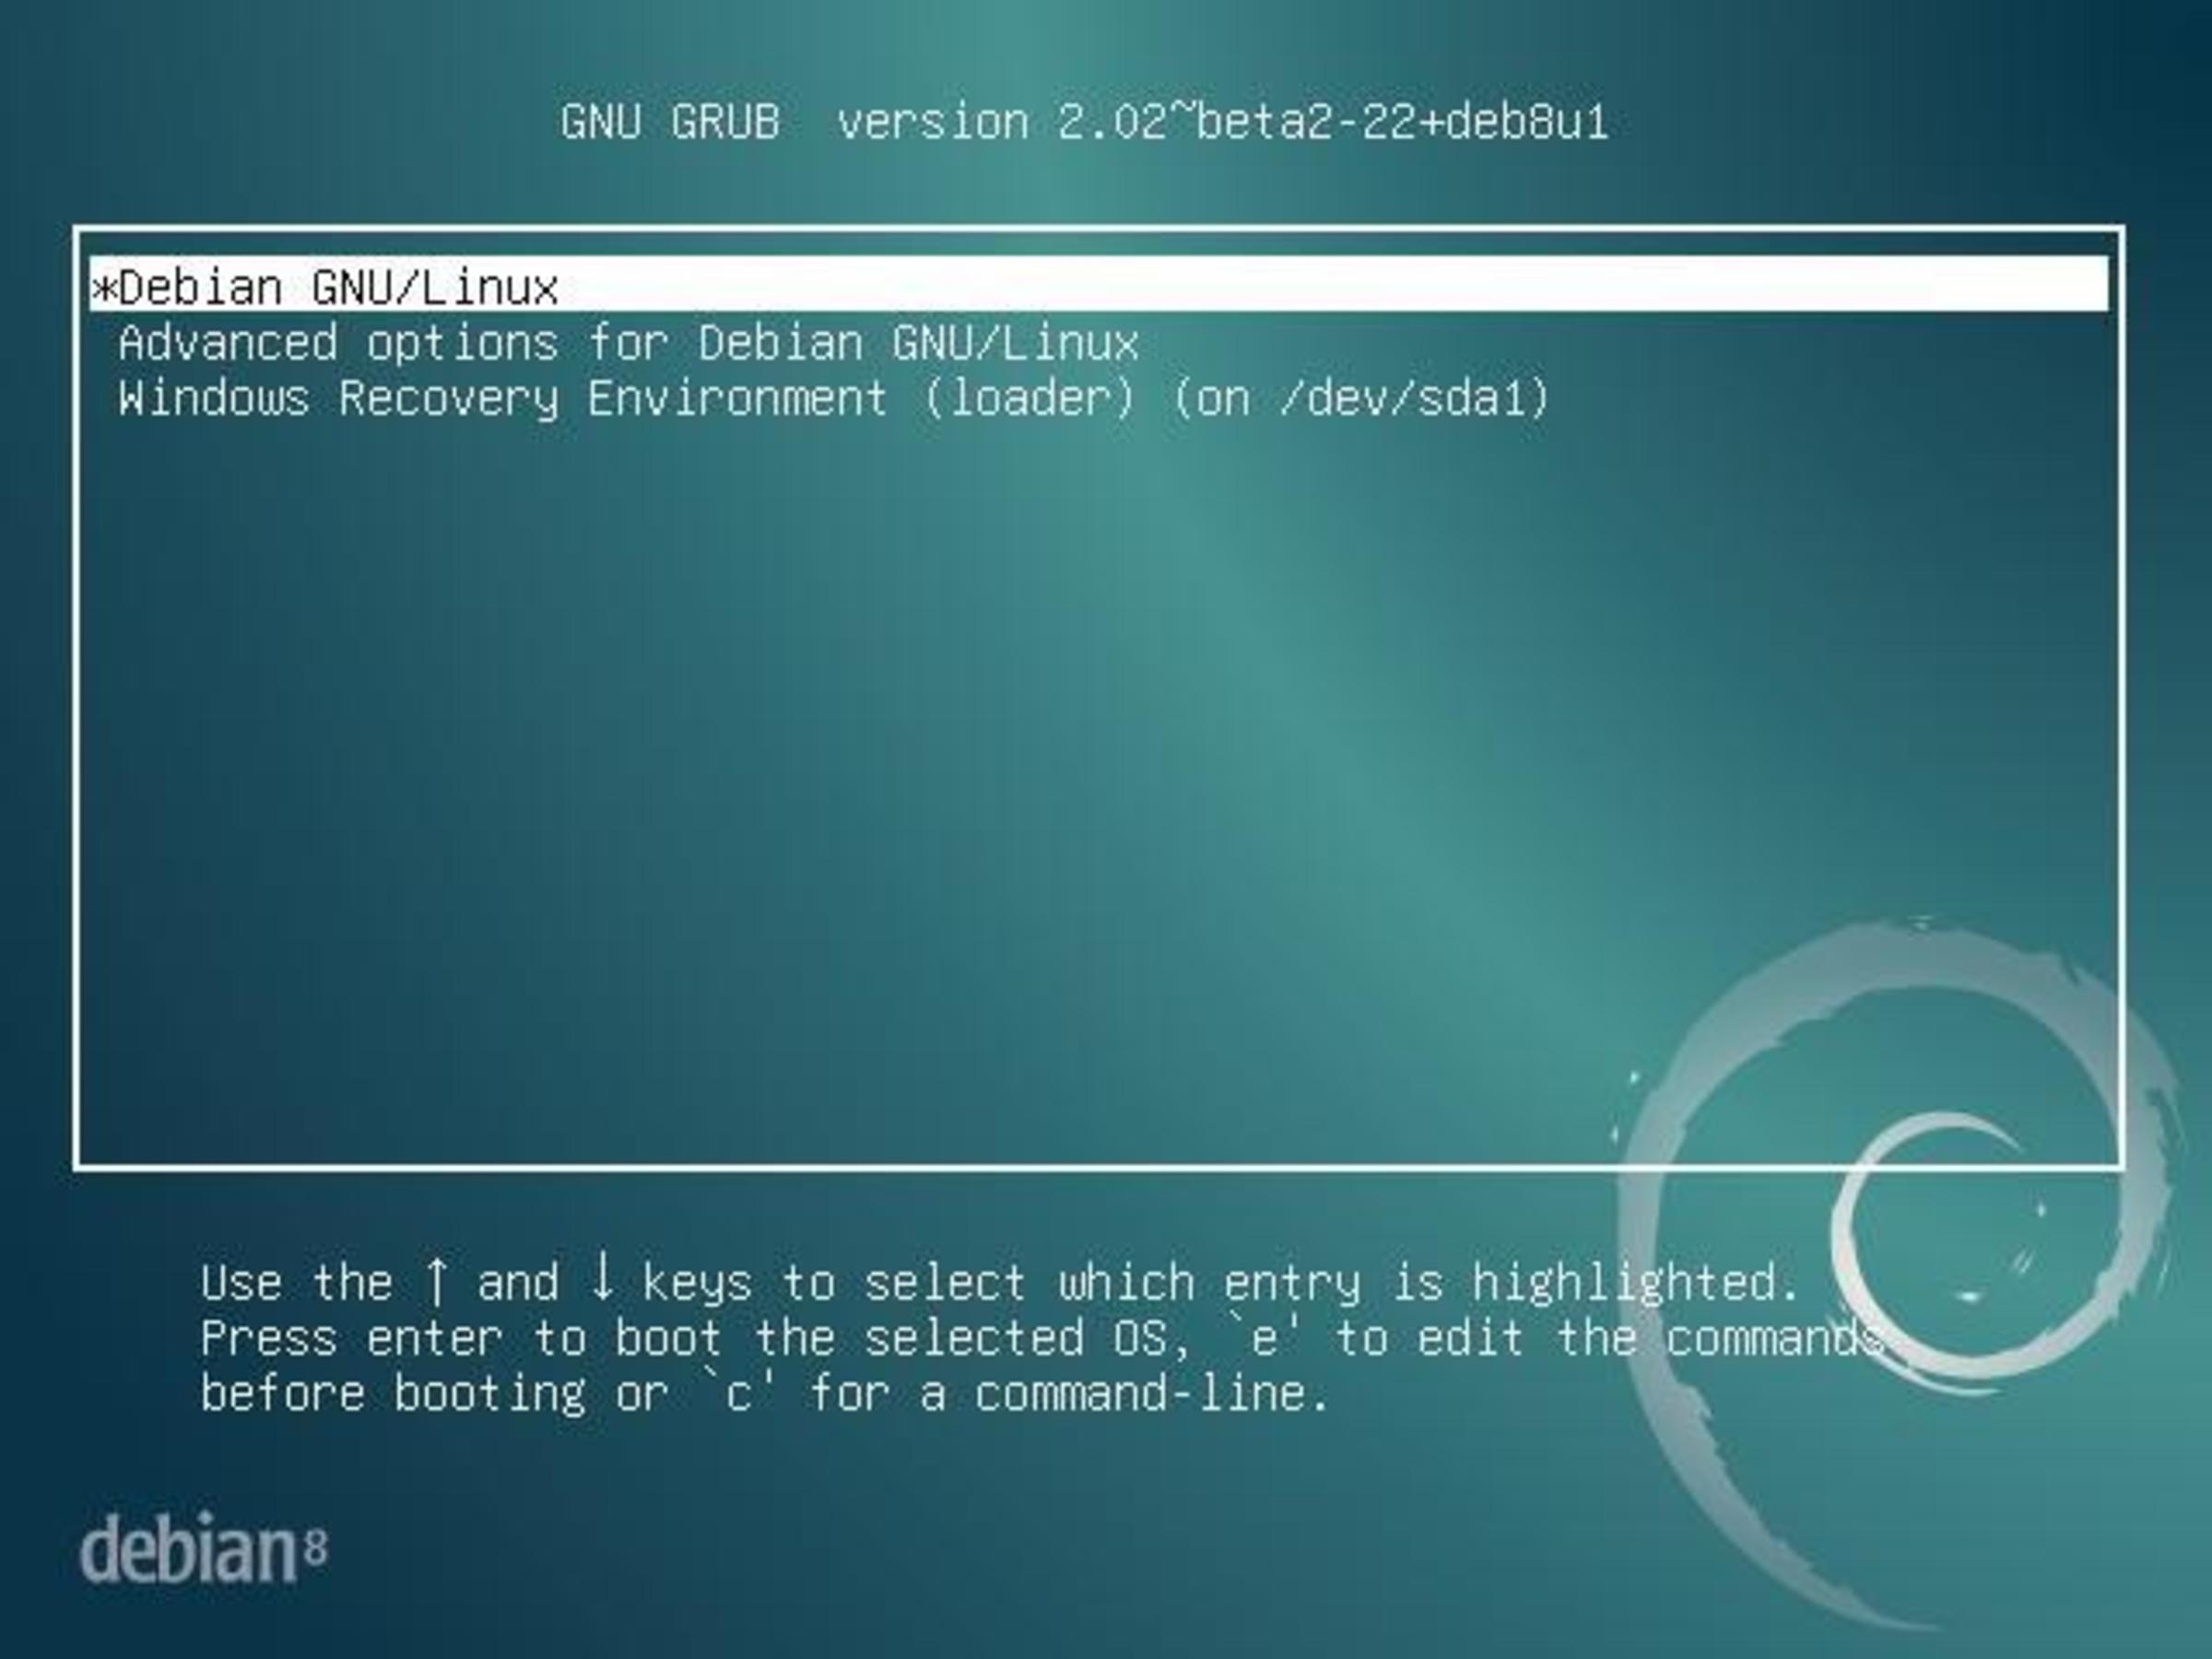
\includegraphics[resolution=600]{grub}
	\caption{Selezione del sistema operativo da avviare con \texttt{GRUB}}
	\label{fig:grub}
\end{figure}


Per avviare Debian, sceglieremo la prima voce. La terza voce altro non è che Windows 10 con un nome un po' fuorviante.

Se tutto funziona, Debian dovrebbe avviarsi e, dopo un po', mostrare la schermata di login. Qui, dobbiamo accedere il nostro \textit{account standard personale}. Non bisogna mai accedere con \texttt{root}! \texttt{root} deve essere utilizzato solo quando strettamente necessario, e sarà possibile passare rapidamente all'account \texttt{root} in qualsiasi momento, anche se si è loggati con l'account standard, con il comando \texttt{su}.


